\begin{minipage}[b]{0.35\textwidth}
In this chapter we study how to derive a model from data, for
example, by fitting a curve to a series of measurements. The
method of least squares is widely used, and gives simple, often
linear algorithms. However, it should be used with care, as it
makes the hidden assumption that error terms are gaussian with
same variance. We also discussed the less known alternative
called $\ell^1$ norm minimization, which implicitly assumes
that error terms have a Laplace instead of gaussian
distribution.
\end{minipage}
%
\begin{minipage}[b]{0.65\textwidth}
\hspace{1cm} ~~~~
\insfig{modfitSigne}{1} ~\\
%~\\
%~\\
%~\\
\end{minipage}
The resulting algorithms may be less simple, but
are often tractable, as they correspond to convex
(rather than linear) optimization, and the method
is more robust to outliers or wrong
distributional assumptions.

We discuss in detail the so-called ``linear
models"; what is linear here is the dependence on
the hidden parameters, not the model itself. This
is a very rich family of models with wide
applicability. We discuss both least square and
$\ell^1$ norm minimization in this context.

Then we discuss the issue of fitting a distribution to a data
set; we describe commonly used features that are helpful to
pick an appropriate distribution: distribution shape, power
laws, fat tail and heavy tail. The latter property is often
encountered in practice and is often interesting or annoying.
We address the practical issues of fitting censored data (i.e.
when we could observe only values smaller than some unknown
threshold) and how to separately fit the body and the tail of a
distribution. We illustrate how the concepts and techniques
could be used to build a load generation tool.
%
\minitoc
%
\section{Model Fitting Criteria}
\subsection{What is Model Fitting~?} We start with a simple
example.
\begin{ex}{Virus Spread Data}\label{ex-virus-spread}
The number of hosts infected by a virus is plotted versus time in
hours.

\Ifig{expoGrowthCharts-Lin}{0.4}{0.3}

The plot suggests an exponential growth, therefore we are inclined
to fit these data to a model of the form
  \be
  Y(t) = a e^{\alpha t} \label{eq-modfit-0}
  \ee
where $Y(t)$ is the number of infected hosts at time $t$. We
are particulary interested in the parameter $\alpha$, which can
be interpreted as the growth rate; the \nt{doubling time} (time
for the number of infected hosts to double) is $\frac{\ln
2}{\alpha}$. On the plot, the dashed line is the curve fitted
by the method of least squares explained later. We find
$\alpha=0.4837$ per hour and the doubling time is $1.43$ hour.
We can use the model to predict that, 6 hours after the end of
the measurement period, the number of infected hosts would be
ca. 82'000.
\end{ex}

In general, \nt{model fitting} can be defined as the problem of
finding an \nt{explanatory model} for the data, i.e. a mathematical
relation of the form
 \be y_i=f_i(\vec{\beta})  \label{eq-modfit-1}\ee
that ``explains the data well", in some sense. Here $y_i$  is the
collection of measured data, $i$ is the index of a measurement,
$f_i$ is an array of functions, and $\vec{\beta}$ is the parameter
that we would like to obtain. In the previous example, the parameter
is $\vec{\beta}=(a, \alpha)$ and $f_i(\vec{\beta})=f_i(a,\alpha)=a
e^{\alpha t_i}$ where $t_i$ is the time of the $i$th measurement,
assumed here to be known.

What does it mean to ``explain the data well"~? It is generally not
possible to require that \eref{eq-modfit-1} holds \emph{exactly} for
all data points. Therefore, a common answer is to require that the
model minimizes some metric of the discrepancy between the
explanatory model and the data. A very common metric is the mean
square distance $\sum_i \left(y_i- f_i(\vec{\beta})\right)^2$. The
value of the growth rate $\alpha$ in the previous example was
obtained in this way, namely, we computed $a$ and $\alpha$ that
minimize $\sum_i (y_i - a e^{\alpha t_i} )^2$.
%
%\mq{q-modfit-klklasd}
% {How would you compute $a$ and  $\alpha$~?}
% {This is a non constrained optimization problem in two variables; we used a generic solver (\pro{fminsearch} in matlab)
% }

But this raises another question. What metric should one use ? What
is so magical about least squares ? Why not use other measures of
discrepancy, for example $\sum_i |y_i - f_i(\vec{\beta})|$ or
$\sum_i \left(\ln(y_i) - \ln(f_i(\vec{\beta}))\right)^2$~? The
following example shows the importance of the issue.

\begin{ex}{Virus Spread Data, Continued. Ambiguity in the Optimization Criterion}
We also plotted the number of infected hosts in log scale:
  \Ifig{expoGrowthCharts-Log}{0.4}{0.3}
and computed the least square fit of \eref{eq-modfit-1} in log
scale (plain line). Namely, we computed $a$ and $\alpha$ that
minimize $\sum_i \left(\ln(y_i) - \ln(a) - \alpha t_i
\right)^2$. We found for $\alpha$ the value $0.39$ per hour,
which gives a doubling time of $1.77$ hour and a prediction at
time $+6$ hours equal to ca. $39'000$ infected hosts (instead
of previously $82'000$).

The two different models are compared below (in linear and log
scales).

\begin{center}
    \Ifignc{expoGrowthCharts-LinBoth}{0.4}{0.3}
    \Ifignc{expoGrowthCharts-LogBoth}{0.4}{0.3}
\end{center}

Both figures show that what visually appears to be a good fit in one
scale is not so in the other. Which one should we use~?
\label{ex-virus-spread-log}
\end{ex}
An answer to the issue comes from statistics. The idea is to add to
the explanatory model a description of the ``noise" (informally
defined as the deviation between the explanatory model and the
data), and obtain a \nt{statistical model}. We can also think of the
statistical model as a description of a simulator that was used to
produce the data we have. Its parameters are well defined, but not
known to us.

The statistical model usually has a few more parameters than the
explanatory model. The parameters of the statistical model are
estimated using the classical approach of maximum likelihood. If we
believe in the statistical model, this answers the previous issue by
saying that the criterion to be optimized is the likelihood. The
belief in the model can be checked by examining residuals.

\begin{ex}{Virus Spread Data, Continued. A Statistical Model} \label{ex-msddsjhkl0}One
\imp{statistical model} for the virus spread data is
 \be
 Y_i = a e^{\alpha t_i} + \epsilon_i  \mbox{    with } \epsilon_i
 \mbox{ iid } \sim N_{0,\sigma^2}
 \label{eq-modfit-askasldk}
 \ee
in other words, we assume that the measured data $y_i$ is equal to
the ideal value given by the explanatory model, plus a noise term
$\epsilon_i$. Further, we assume that all noises are independent,
gaussian, and with same variance. The parameter is $\theta=(a,
\alpha, \sigma)$.

In \eref{eq-modfit-askasldk}, we write $Y_i$ instead of $y_i$ to
express that $Y_i$ is a random variable. We think of our data $y_i$
as being \emph{one} sample produced by a simulator that implements
\eref{eq-modfit-askasldk}.

We will see in \sref{sec-lshomo} that the maximum likelihood
estimator for this model is the one that minimizes the mean square
distance. Thus, with this model, we obtain for $\alpha$ the value in
\exref{ex-virus-spread}.

A second statistical model could be:
 \be
  \ln(Y_i) = \ln\left(a e^{\alpha t_i}\right) + \epsilon_i
  \mbox{    with } \epsilon_i
 \mbox{ iid } \sim N_{0,\sigma^2}
 \label{eq-modfit-askasldkaa}
 \ee
Now, we would be assuming that the noise terms in log-scale have the
same variance, in other words, the noise is proportional to the
measured value. Here too, the maximum likelihood estimator is
obtained by minimizing the least square distance, thus we obtain for
 $\alpha$ the value in \exref{ex-virus-spread-log}.


We can validate either model by plotting the residuals:
\begin{center}
    \Ifignc{expoGrowthResiduals-Lin}{0.4}{0.3}
    \Ifignc{expoGrowthResiduals-Log}{0.4}{0.3}
\end{center}
We see clearly that the residual for the former model do not appear
to be normally distributed, and the converse is true for the former
model, which is the one we should adopt. Therefore, an acceptable
fitting is obtained by minimizing least squares in
log-scale.
 %\mq{q-modfit-kklasdkl}
% {How would you compute the residuals~?}
% {The
%residuals are estimates of the noise terms $\epsilon_i$. Let
%$\hat{a}$ and $\hat{\alpha}$ be the values estimated by maximum
%likelihood, for either model. The residuals are $r_i= y_i -\hat{a}
%e^{\hat{\alpha} t_i}$ for the former model, $r_i= \ln y_i
%-\ln\left(\hat{a} e^{\hat{\alpha} t_i}\right)$ for the latter. }
\end{ex}

We summarize what we have learnt so far as follows.

\begin{sh}
\paragraph{Fitting a Model to Data}
\begin{enumerate}
    \item Define a statistical model that contains \imp{both} the
    deterministic part (the one we are interested in) and a model of
    the noise.
    \item Estimate the parameters of the statistical model using
    maximum likelihood. If the number of data points is small, use a
    brute force approach (e.g use \pro{fminsearch}). If the number
    of data points is large, you may need to look in the literature
    for efficient, possibly heuristic, optimization methods.
    \item Validate the model fit by screening the residuals, either
    visually, or using tests (\cref{ch-tests}).
    In practice, you will seldom obtain a perfect
    fit; however, large deviations indicate that
    the model might not be appropriate.
\end{enumerate}
\end{sh}
\subsection{Least Squares Correspond to Gaussian, Same Variance}
\label{sec-lshomo} A very frequent case is when the statistical
model has the form
 \be
 Y_i = f_i(\vec{\beta}) + \epsilon_i \mfor i=1,\ldots,I \mbox{    with } \epsilon_i
 \mbox{ iid } \sim N_{0,\sigma^2}
 \label{eq:ls-mod}
 \ee
as in the examples before (Models in
Equations~(\ref{eq-modfit-askasldk}) and
(\ref{eq-modfit-askasldkaa})). Namely, the discrepancy between the
 explanatory model and the data is assumed to be gaussian with
 \imp{same variance}. In some
literature, the ``same variance" assumption is called
\nt{homoscedasticity}.


The next theorem explains what we do when we fit the
explanatory model $y_i= f_i(\vec{\beta})$ to our data using
least squares: we implicitly assume that the error terms in our
data are independent, gaussian, and of same amplitude. We have
seen in the examples above that care must be taken to validate
this assumption, in particular, some rescaling may be needed
for a better validation.

\begin{shadethm}[Least Squares]  For the model in \eref{eq:ls-mod},
\begin{enumerate}
    \item the maximum likelihood estimator of the parameter
        $(\vec{\beta},\sigma)$ is given
        by:\begin{enumerate}
    \item
$\hat{\beta}  = \arg\min_{\vec{\beta}} \sum_{i} \left(y_i -
f_i(\vec{\beta})\right)^2$
    \item
$\hat{\sigma}^2=\frac{1}{I}\sum_i\left(y_i
-f_i(\hat{\beta})\right)^2$
\end{enumerate}

\item Let $K$ be the square
    matrix of second derivatives (assumed to exist), defined by
    \ben
    K_{j,k} = \frac{1}{\sigma^2}\sum_i\pder{f_i}{\beta_j}\pder{f_i}{\beta_k}
    \een
    If $K$ is invertible and if the
    number
    $I$
    of
    data
    points
    is
    large,
    $\hat{\beta}-\vec{\beta}$ is approximately gaussian with
    $0$ mean and covariance matrix $K^{-1}$.


Alternatively, for large $I$, an approximate confidence set at
level $\gamma$ for the $j$th component
  $\beta_j$ of $\vec{\beta}$ is implicitly defined by
 \ben
 -2 I\ln \lp \hat{\sigma}\rp +2 I\ln \lp \hat{\sigma}(\hat{\beta}_1,...,\hat{\beta}_{j-1},\beta_j,\hat{\beta}_{j+1}...\hat{\beta}_p)\rp
 \geq \xi_1
  \een
  where $\hat{\sigma}^2(\vec{\beta})=\frac{1}{I}\sum_i\lp y_i- f_i(\vec{\beta})\rp^2$
  and $\xi_1$ is the $\gamma$ quantile of the $\chi^2$
  distribution with 1 degree of freedom (for example, for $\gamma= 0.95$,
  $\xi_1=3.92$).
  \end{enumerate}
\label{theo-lslls}
\end{shadethm}


The set of points in $\Reals^I$ that have coordinates of the
form $f_i(\vec{\beta})$ constitue a ``manifold" (for $p=2$, it
is a surface). Item 1~(a) says that $\vec{\beta}$ is the
parameter of the point $\hat{y}$ on this manifold that is the
nearest to the data point $\vec{y}$, in euclidian distance. The
point $\hat{y}$ is called the \nt{predicted response}; it is an
estimate of the value that $\vec{y}$ would take if there would
be no noise. It is equal to the orthogonal projection of the
data $\vec{y}$ onto the manifold.

The rest of the theorem can be used to obtain
accuracy bounds for the estimation. A slight
variant of the theorem can be used to make
predictions with accuracy bounds, see
\thref{theo-lr-pi}.

%\mq{q-modfit-ldslsadlk99}{How would you compute confidence intervals
%for $\vec{\beta}~?$} {One method is to use the asymptotic confidence
%interval of \thref{theo-mle}. A second method is the bootstrap: draw
%$R$ bootstrap replicates of $\vec{Y}$ and obtain $R$ estimates of
%$\vec{\beta}$. Use the order statistics of the bootstrap estimates
%to obtain confidence intervals.}


%\nfs{
\subsection{$\ell^1$ Norm
Minimization Corresponds to Laplace Noise}

Although less traditional than least square,
minimization of the absolute deviation of the
error is also used. The absolute deviation is the
$\ell^1$ norm of the error\footnote{The $\ell^1$
norm of a sequence $z=(z_1,...,z_n)$ is
$\norm{z}_1=\sum_{i=1}^n \abs{z_i}$}, so this
method is also called \nt{$\ell^1$ norm
minimization}. Since it gives less weight to
outliers, it is expected to be more robust. As we
see now, it corresponds to assuming that errors
follow a Laplace distribution (i.e. bilateral
exponential).

The \nt{Laplace distribution}\label{def-laplace}
with $0$ mean and rate $\lambda$ is the two sided
exponential distribution, or, in other words, $X
\sim \mbox{
 Laplace}(\lambda)$ if and only if $\abs{X}\sim \mbox{Exp}(\lambda)$.
It can be used to model error terms that have a heavier tail
 than the normal distribution. Its PDF is defined for $x \in
 \Reals$ by
 \be
 f(x)= \frac{\lambda}{2}e^{-\lambda\abs{ x}}
 \ee
%
The next theorem explains what we do when we fit
the explanatory model $y_i= f_i(\vec{\beta})$ to
our data by minimizing the $\ell^1$ norm of the
error: we implicitly assume that the error terms
in our data are independent, Laplace with the
same parameter, i.e., the data $yy_i$ is a sample
generated by the model
\be
 Y_i = f_i(\vec{\beta}) + \eps_i \mbox{ with } \eps_i \mbox{iid} \sim \mbox{
 Laplace}(\lambda) \label{eq:ld-mod}
 \ee
\begin{shadethm}[Least Deviation] For the model in \eref{eq:ld-mod},
the maximum likelihood estimator of the parameter
$(\vec{\beta},\la)$ is given by:\begin{enumerate}
    \item
$\hat{\beta}  = \arg\min_{\vec{\beta}} \sum_{i} \abs{y_i -
f_i(\vec{\beta})}$
    \item
$\frac{1}{\hat{\la}}=\frac{1}{I}\sum_i\abs{y_i
-f_i(\hat{\beta})}$
\end{enumerate}
%
 \label{theo-ladlls}
\end{shadethm}

\begin{figure}[htbp]
\begin{center}
    \Ifignc{expoGrowthCharts-Log-noOut-GL}{0.4}{0.3}
    \Ifignc{expoGrowthCharts-Log-out3-GL}{0.4}{0.3}
\end{center}
% sources: expoGro.dat, expoGroOutlier3.dat, fitExpo.m and fitLaplaceToExpGro.m
\label{fig-laplace-expoGro-GL} \mycaption{Fitting
an exponential growth model to the data in
\exref{ex-virus-spread}, showing the fits
obtained with least square (plain) and with
$\ell^1$ norm minimization (dashed) . First
panel: original data; both fits are the same;
Second panel: data corrupted by one outlier;
the fit with $\ell^1$ norm
minimization is not affected, whereas the least
square fit is.}
\end{figure}
\begin{ex}{Virus Propagation with One Outlier}
Assume the data in the virus propagation example
(\exref{ex-virus-spread}) is modified by changing
the value of the second data point. Assume we fit
the data in log scale. The modified data is an
outlier; perhaps one would be tempted to remove
it; an alternative is to fit the log of the data
to Laplace noise instead of gaussian noise (i.e.
do $\ell^1$ norm minimization instead of least
squares), as this is known to be more robust.
\fref{fig-laplace-expoGro-GL}, and the table
below shows the results (the prediction in the
table is a 6-hours ahead point prediction).

\vspace{0.7cm}
 \begin{tabular}{|r|c|c|c|c|}
   % after \\: \hline or \cline{col1-col2} \cline{col3-col4} ...
  %
   \hline
    & \multicolumn{2}{c|}{Least Square } & \multicolumn{2}{c|}{$\ell^1$ norm minimization}
    \\
    \cline{2-5}
    & rate   &  prediction & rate &   prediction \\
     \hline \hline
   no outlier & 0.3914  &     30300 & 0.3938 &    32300 \\
   \hline
   with one outlier&0.3325  &   14500 & 0.3868 &
   30500\\
   \hline
  %
 \end{tabular}
\vspace{0.7cm}

We see that one single outlier completely
modifies the result of least square fitting,
whereas $\ell^1$ norm minimization fitting is not
impacted much.
\end{ex}

The following example is important to understand
the difference between least square and $\ell^1$
norm minimization.
\begin{ex}{Mean versus Median}Assume we want to
fit a data set $y_i$,  $i=1,...,I$ against a
constant $\mu$.

With least square fitting, we are looking for
$\mu$ that minimizes $\sum_{i=1}^I \lp y_i -\mu
\rp^2$. The solution is easily found to be
$\mu=\frac{1}{I}\sum_{i=1}^I y_i$, i.e. $\mu$ is
the sample mean.

With $\ell^1$ norm minimization, we are looking
for $\mu$ that minimizes $\sum_{i=1}^I \abs{ y_i
-\mu }$. The solution is the median of $y_i$.

To see why, consider the mapping $f: \mu \mapsto \sum_{i=1}^I
\abs{ y_i -\mu }$. Consider to simplify the case where all
values $y_i$ are distinct and written in increasing order
($y_i< y_{i+1}$). The derivative $f'$ of $f$ is defined
everywhere except at points $y_i$, and for $y_i < \mu
<y_{i+1}$, $f'(\mu) = i - (I-i)= 2i-I$. If $I$ is odd, $f$
decreases on $(-\infty, y_{(I+1)/2}]$ and increases on
$[y_{(I+1)/2}, +\infty)$, thus is minimum for $\mu=
y_{(I+1)/2}$, which is the sample median. If $I$ is even, $f$
is minimum at all values in the interval $[y_{I/2}, y_{I/2+1}]$
thus reaches the minimum at the sample median $\frac{y_{I/2},
y_{I/2+1}}{2} $. \label{ex-mean-median}
\end{ex}

In terms of computation, $\ell^1$ norm
minimization is more complex than least squares,
though both are usually tractable. For example,
if the dependency on the parameter is linear,
least square fitting consists in solving a linear
system of equations whereas $\ell^1$ norm
minimization uses linear programming (as shown in
the next section).

\section{Linear Regression}
\mylabel{sec-lrn} This is a special case of least
square fitting, where the explanatory model
depends linearly on its parameter $\vec{\beta}$.
This is called the \nt{linear regression} model.
The main fact here is that everything can be
computed easily, using linear algebra. Be careful
that the term ``linear regression" implicitly
assumes least square fitting. The popular fitting
method called ``ANOVA" is a special case of
linear regression.

Assume thus that the \emph{statistical model} of our experiment has
the form:\\
\begin{sh}
\begin{definition}[Linear Regression Model] \label{def:ls:lin}
 \be
 Y_i = (X \vec{\beta})_i + \epsilon_i \mfor i=1,\ldots,I \mbox{    with } \epsilon_i
 \mbox{ iid } \sim N_{0,\sigma^2}
 \label{eq-def-lr}
 \ee
where the unknown parameter $\vec{\beta}$ is in $\Reals^p$ and $X$
is a $I\times p$ matrix. The matrix $X$ supposed to be known exactly
in advance. We also assume that
\begin{description}
    \item[H]  $X$ has rank $p$
\end{description}
\end{definition}
\end{sh}

Assumption \textbf{H} means that different values of $\vec{\beta}$
give different values of the explanatory model $X \vec{\beta}$, i.e.
the explanatory model is identifiable.

The elements of the known matrix $X$ are sometimes called
\nt{explanatory variables}, and then the $y_i$s are called the
\nt{response variables}.


\begin{ex}{Joe's Shop again, \fref{metho-f2}}\label{ex-5-3}
\label{ex-joe-again-modfit} We assume that there is a threshold
$\xi$ beyond which the throughput collapses (we take
 $\xi=70$). The statistical model is
 \be
Y_i= (a + b x_i) 1_{x_i \leq \xi} + (c + d x_i) 1_{\{x_i >
\xi\}} + \epsilon_i
 \mylabel{eq-factors-ia}
 \ee
 where we impose
\begin{equation}\mylabel{eq-relx3-f0}
  a + b\xi=c + d\xi
\end{equation}
In other words, we assume the throughput response curve to be
piecewise linear. \eref{eq-relx3-f0} expresses that the curve is
continuous. Recall that $x_i$ is the offered load and $Y_i$ is the
actual throughput.

Here we take $\vec{\beta}=(a,b,d)$ (we can derive $c=a +
(b-d)\xi$ from \eref{eq-relx3-f0}). The dependency of $Y_i$ on
$\vec{\beta}$ is indeed linear. Note that we assume that $\xi$
is known; see in \exref{ex-joe-nonline} how to estimate $\xi$.

Assume that we sort the $x_i$s in increasing order and let $i^*$ be
the largest index $i$ such that $x_i \leq \xi$. Re-write
\eref{eq-factors-ia} as
 \bearn
Y_i&=& a + b x_i + \epsilon_i  \mfor i=1 \ldots i^*\\
Y_i &=& a + b\xi + d (x_i-\xi) + \epsilon_i  \mfor i=i^*+1 \ldots I
 \eearn
thus the matrix $X$ is given by:
 \ben
 \bmat{c c c}
 \\
1 & x_1 & 0 \\
1 & x_2 & 0 \\
\cdots & \cdots &\cdots \\
1 & x_{i^*} & 0\\
1 & \xi &  x_{i^*+1}-\xi \\
\cdots  &\cdots &\cdots \\
1 & \xi &  x_{I}-\xi \\
 \emat
 \een

It is simple to see that a \emph{sufficient} condition for
\textbf{H} is that there are at least two distinct values of $x_i
\leq \xi$ and at least one value $>\xi$.

\mq{q-modfit-dsasadj}{Show this.} {We need to show, if the condition
is true, that the matrix $X$ has rank $p=3$. This is equivalent to
saying that the equation
 \ben
 X \bmat{c}a\\b\\d\emat  = 0
 \een
has only the solution $a=b=d=0$. Consider first $a$ and $b$. If
there are two distinct values of $x_i$, $i \leq i^*$, say $x_1$ and
$x_2$ then $a +bx_1=a+b x_2=0$ thus $a=b=0$. Since there is a value
$x_i >\xi$, it follows that $i^*+1\leq I$ and $d (x_{I}-\xi)=0$ thus
$d=0$.} A model as in this example is sometimes called
\nt{Intervention Analysis}.
\end{ex}

With the linear regression model, the manifold mentioned in the
discussion after \thref{theo-lslls} is a linear manifold (for
$p=2$, a plane). It is equal to the linear sub-space spanned by
the columns of matrix $X$. The nearest point is given by an
orthogonal projection, which can be computed exactly. The
details are given in the following theorem which is a
consequence of \eref{eq-proj-orth-im} on
\pgref{eq-proj-orth-im} and \thref{theo-homsced}; a complete
proof is in \cite[section 2.3]{davison2003sm}.

\begin{shadethm}[Linear Regression]
Consider the model in Definition~\ref{def:ls:lin}; let $\vec{y}$ be
the $I\times1$ column vector of the data.
 \begin{enumerate}
  \item The $p\times p$ matrix $(X^T X)$ is invertible
  \item (Estimation) The maximum likelihood estimator of $\vec{\beta}$ is
  $\hat{\beta}=K \vec{y}$ with $K=(X^T X)^{-1}X^T$
  \item (Standardized Residuals) Define the $i$th residual as
 $e_i= \left(\vec{y}- X\hat{\beta}\right)_i$. The residuals are zero-mean gaussian but are
correlated, with covariance matrix $\sigma^2 (Id_I -H)$, where
 $H=X (X^T X)^{-1}X^T$.

Let
 $s^2=\frac{1}{I-p}\norm{e}^2=\frac{1}{I-p}\sum_i e_i^2$ (rescaled sum of squared
 residuals). $s^2$ is an unbiased estimator of $\sigma^2$.


 The standardized residuals defined by $r_i:=\frac{e_i}{s
  \sqrt{1-H_{i,i}}}$ have unit variance and $r_i \sim
  t_{I-p-1}$. This can be used to test the model by
  checking that $r_i$ are approximately normal with unit
  variance.
  \item (Confidence Intervals)
  Let $G=\left(X^T X\right)^{-1}=KK^T$; the distribution of $\hat{\beta}$ is gaussian with mean
$\vec{\beta}$ and covariance matrix $\sigma^2 G$, and
$\hat{\beta}$ is independent of $e$.

In particular, assume we want a confidence interval for a (non-random) linear combination of the parameters $\gamma=\sum_{j=1}^{p} u_j \beta_j$;
 $\hat{\gamma}=\sum_j
u_j\hat{\beta}_j$ is our estimator of $\gamma$. Let
% be a (non-random)
%linear combination of the parameter
%$\vec{\beta}$; $\hat{\gamma}=\sum_j
%u_j\hat{\beta}_j$ is our estimator of $\gamma$.
%Let $G=\left(X^T X\right)^{-1}=KK^T$
%and
$g=\sum_{j,k}u_j G_{j,k} u_k=\sum_k
\left(\sum_j u_j K_{j,k} \right)^2$ ($g$ is
called the \nt{variance bias}). Then $
\frac{\hat{\gamma}-\gamma}{\sqrt{g}s} \sim
t_{I-p} $. This can be used to obtain a
confidence interval for $\gamma$.
 \end{enumerate}
 \label{theo:lr}
\end{shadethm}
%Let $g=\sum_k \left(\sum_j u_j K_{j,k} \right)^2$
%(\nt{variance bias}).
%
%
%Remplacer peut etre par :$\cov(\hat{\beta})=\sigma^2 (X^T
%X)^{-1}$

\textbf{Comments. }
Item 4 is often used as follows : if we ignore the uncertainty due to the estimation of $\sigma$, the estimation error (in estimating $\vec{\beta}$) is approximately gaussian with covariance matrix $G$ (sometimes called the ``variance-covariance matrix").


Item 3 states that the residuals are
(slightly) biased, and it is better to use standardized
residuals.

The matrix $H$ is the projection onto the subspace spanned by
the columns of $X$ (\eref{eq-proj-orth-im} on
\pgref{eq-proj-orth-im}). The predicted response is $\hat{y}=X
\hat{\beta}$. It is equal to the orthogonal projection of
$\vec{y}$, and is given by
 \be \hat{y}=H\vec{y} \label{eq:predresp:lin}\ee

The scaled sum of squared residuals $s^2$ is also equal to
$\frac{1}{I-p}\left(\norm{\vec{y}}^2- \norm{\hat{y}}^2\right)$.
Its distribution is $\frac{1}{I-p}\chi^2_{I-p}$. This can be
used to compute a confidence interval for $\sigma$.


%The proof of the theorem shows a slightly stronger result than item
%4: the joint distribution of $\hat{\beta}$ is gaussian with mean
%$\vec{\beta}$ and covariance matrix $\sigma^2 K K^T$, and
%$\hat{\beta}$ is independent of $e$.

\begin{ex}{Joe's Shop again. Continuation of Example~\ref{ex-joe-again-modfit}}
We can thus apply matrix computations given in \thref{theo:lr}; item
2 gives an estimate of $(a,b,d)$ and thus of $c$. Item 4 gives
confidence intervals. The values and the fitted linear regression
model are shown in the table and figure below.
%\begin{figure}[!htbp]
\begin{center}

%  \mycaption{ fitted to \exref{ex-5-3}.}
%  \mylabel{fig-relx3}
%\end{figure}

%\begin{table} \label{tab-relx3}
%  \centering
\begin{tabular}[b]{cc} \hline
  % after \\ : \hline or \cline{col1-col2} \cline{col3-col4} ...
  a & $0.978 \pm 0.609$ \\
  b & $0.0915 \pm 0.0137$ \\
  c & $15.8 \pm 2.99$ \\
  d & $-0.121 \pm 0.037$ \\ \hline
\end{tabular}
\Ifignc{ex53}{0.6}{0.4}
\end{center}
 %\mycaption{Confidence intervals for $a,b,c,d$ in \exref{ex-5-3}.}
%\end{table}
We also computed the residuals $e_i$ (crosses) and standardized
residuals $r_i$ (circles). There is little difference between both
types of residuals. They appear reasonably normal, but one might
criticize the model in that the variance appears smaller for smaller
values of $x$.  The normal qqplot of the residuals also shows
approximate normality (the qqplot of standardized residuals is
similar and is not shown).
 \begin{center}
  \Ifignc{joeResiduals}{0.4}{0.27}
  \Ifignc{joeResidualsQq}{0.4}{0.3}
 \end{center}

 \mq{q-skjsdakj}{Can we conclude that there is congestion collapse~?}{Yes, since the confidence
 interval for  $d$ is entirely positive [resp. negative].}
\label{ex-joe-jjjj}
\end{ex}
\paragraph{Where is Linearity~?}
In the previous example, we see that that $y_i$ is a linear function
of $\vec{\beta}$, but \imp{not of $x_i$}. This is quite general, and
you should avoid a widespread confusion:  linear regression is not
restricted to models where the data $y_i$ is linear with the
explanatory variables $x_i$.

%\paragraph{Beyond the Linear Case}
\begin{ex}{Joe's Shop - Beyond the Linear Case - Estimation of
$\xi$}\label{ex-joe-nonline} In \exref{ex-5-3} we assumed that
the value $\xi$ after which there is congestion collapse is
known in advance. Now we relax this assumption. Our model is
now the same as \eref{eq-factors-ia}, except that $\xi$ is also
now a parameter to be estimated.

To do this, we apply maximum likelihood estimation. We have to
maximize the log-likelihood $l_{\vec{y}}(a,b,d,\xi,\sigma)$, where
$\vec{y}$, the data, is fixed. For a fixed $\xi$, we know the value
of $(a,b,d,\sigma)$ that achieves the maximum, as we have a linear
regression model. We plot the value of this maximum versus $\xi$
(\fref{fig-josagain-kklw}) and numerically find the maximum. It is
for $\xi=77$.

To find a confidence interval, we use the asymptotic result in
\thref{theo-mle2}. It says that a  $95\%$ confidence interval is
obtained by solving $l(\hat{\xi}) - l(\xi) \leq 1.9207$, which gives
 $\xi \in [73,80]$. %The fitted model and its residuals are shown in
% \fref{fig:regress1}.
\end{ex}
\begin{figure*}[htb!]
  \begin{center}
    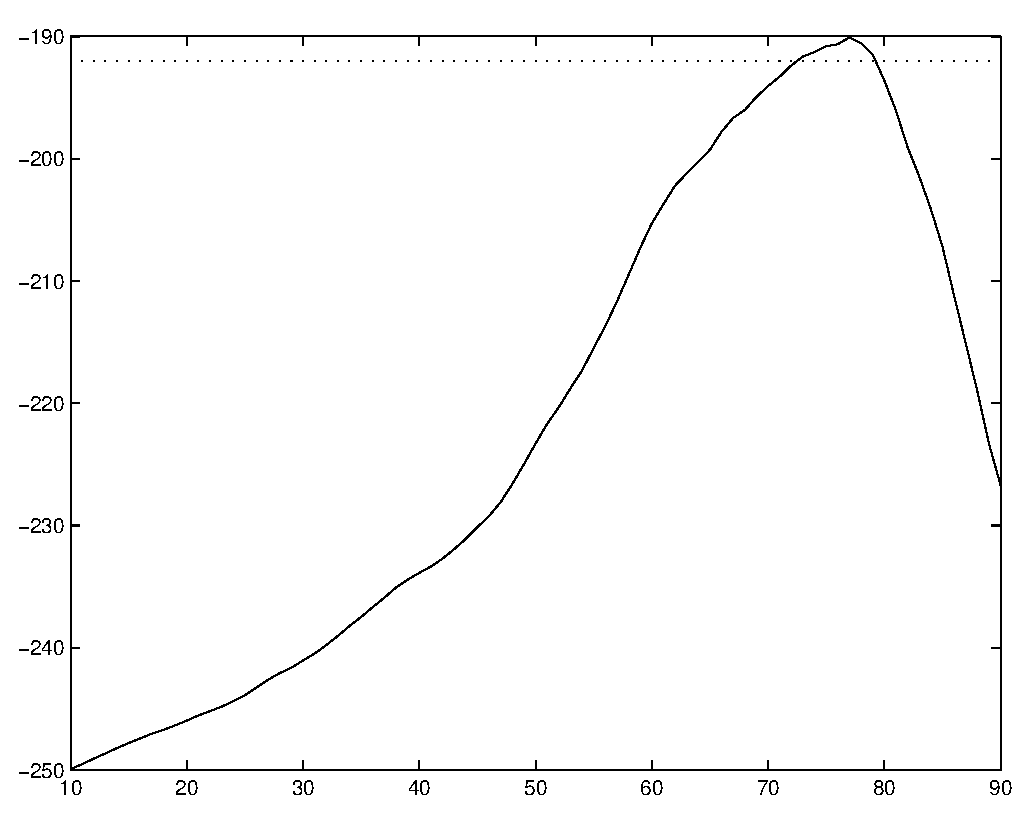
\includegraphics[angle=0,scale=0.6]{hw54a.eps}
    \mycaption{Log likelihood for Joes' shop as a function of $\xi$.\label{fig-josagain-kklw}}
  \end{center}
\end{figure*}


\section{Linear Regression with $\ell^1$ Norm Minimization}
This is a variant of the linear regression model,
but with Laplace instead of Gaussian noise. The
theory is less simple, as we do not have explicit
linear expressions. Nonetheless, it uses linear
programming and is thus often tractable, with the
benefit of more robustness to outliers.

The \emph{statistical model} of our experiment
has
the form:\\

\begin{definition}[Linear Regression Model with Laplace Noise] \label{def:lad:lin}
 \be
 Y_i = (X \vec{\beta})_i + \epsilon_i \mfor i=1,\ldots,I \mbox{    with } \epsilon_i
 \mbox{ iid } \sim \mbox{ Laplace }(\la)
 \label{eq-def-lr-lap}
 \ee
where the unknown parameter $\vec{\beta}$ is in
$\Reals^p$ and $X$ is a $I\times p$ matrix. The
matrix $X$ supposed to be known exactly in
advance. As in \sref{sec-lrn}, we assume that $X$
has rank $p$, otherwise the model is non
identifiable.
\end{definition} The following is
an almost immediate consequence of
\thref{theo-ladlls}.

\begin{theorem} Consider the model in Definition~\ref{def:ls:lin}; let $\vec{y}$ be
the $I\times1$ column vector of the data. The
maximum likelihood estimator of $\vec{\beta}$ is
obtained by solving the linear program:
 \bearn
 \mbox{ minimize } &&\sum_{i=1}^I u_i
 \\
\mbox{over } &&\vec{\beta} \in \Reals^p, u \in
 \Reals^I\\
 \\
 \mbox{ subject to the constraints }&& u_i \geq
 y_i -\lp X \vec{\beta}\rp_i\\
&& u_i \geq
 -y_i +\lp X \vec{\beta}\rp_i
 \eearn
The maximum likelihood estimator of the noise parameter
$\la$ is $\lp \frac{1}{I}\sum_{i=1}^I\abs{y_i
-\lp X \vec{\beta}\rp_i} \rp^{-1}$.
 \label{theo-lr-l1}
\end{theorem}

In view of \exref{ex-mean-median}, there is
little hope to obtain nice closed form formulas
for confidence intervals, unlike what happens
with the least square method in \thref{theo:lr},
and indeed the theorem does not give any. To
compute confidence intervals, we can use the
bootstrap, with re-sampling from residuals, as
described in \aref{algo-bs-sr}.

%%%% algorithm for computing confidence interval for $\vec{beta}$.

\begin{algorithm}\mycaption{The Bootstrap with Re-Sampling From
Residuals. The goal is to compute a confidence
interval for some function $\varphi(\vec{\beta})$
of the parameter of the model in
Definition~\ref{def:ls:lin}. $r_0$ is the
algorithm's accuracy parameter.}
 \begin{algorithmic}[1]
%
  \State $R=\lceil 2 \;r_0/(1-\gamma)\rceil-1$  \Comment{For example
  $r_0=25$, $\gamma=0.95$, $R=999$}
%
\State estimate $\vec{\beta}$ using
\thref{theo-lr-l1}; obtain $\hat{\beta}$
%
\State compute the residuals $e_i=y_i -\lp X
\hat{\beta}\rp_i$
%
    \For{$r=1:R$} \Comment{Re-sample from
    residuals}
    \State draw $I$ numbers with replacement from
the list $(e_1, ...,e_I)$ and call them
$E^r_{1},...,E^r_{I}$
    \State generate the bootstrap replicate
    $Y^r_{1},...,Y^r_{I}$ from the estimated
    model:
    \State ~~~~~ $Y^r_i = \lp X \hat{\beta}\rp_i
    + E^r_i $ for $i=1...I$
    \State re-estimate $\vec{\beta}$, using $Y^r_i$ as data, using \thref{theo-lr-l1}; obtain $\vec{\beta}^r$
  \EndFor
  \State $\left(\varphi_{(1)},...,\varphi_{(R)}\right)=\mbox{sort}\left(\varphi(\vec{\beta}^1) ,...,\varphi(\vec{\beta}^R)\right)$
  \State confidence interval for $\varphi(\vec{\beta})$ is
  $[\varphi_{(r_0)}\;;\;\varphi_{(R+1-r_0)}]$ \
\end{algorithmic}\label{algo-bs-sr}
 \end{algorithm}

Note that the algorithm applies to any model
fitting method, not just to models fitted with
\thref{theo-lr-l1}. As always with the bootstrap,
it provides approximate confidence intervals,
with a tendency to underestimate.


\begin{figure}[htb]
\begin{center}
\subfigure[Best fit]
 {\Ifignc{joeLinearFitLAD}{0.4}{0.3}\label{joe-LAD-fit}}
\subfigure[Score versus $\xi$]
  {\Ifignc{joeLinearFitResidualsLADScore}{0.4}{0.3}\label{joe-LAD-s}}
\subfigure[Residuals]
 {\Ifignc{joeLinearFitResidualsLAD}{0.4}{0.3}\label{joe-LAD-res}}
\subfigure[Laplace QQ-plot of Residuals]
 {\Ifignc{joeLinearFitResidualsLaplacePlotLAD}{0.4}{0.3}\label{joe-LAD-qq}}
\end{center}
\mycaption{Modelling congestion collapse in Joe's
shop with a piecewise linear function and
$\ell^1$ norm minimization of the errors.}
\end{figure}

\begin{ex}{Joe's shop with $\ell^1$ norm minimization}
We revisit \exref{ex-5-3} and estimate a piecewise linear
throughput response (as in \eref{eq-factors-ia}) with $\ell^1$
norm minimization, i.e. assuming the error terms $\epsilon_i$
come from a Laplace distribution.

The problem is linear and has full rank if we
take as parameter for example $(a,b,c)$, but it
is not linear with respect to $\xi$. To overcome
this issue, we first estimate the model,
considering $\xi$ as fixed, using linear
programming. Then we vary $\xi$ and look for the
value of $\xi$ that maximizes the likelihood.

In \fref{joe-LAD-s} we plot $\xi$ versus the
score ($\ell^1$ norm of the error). By
\thref{theo-ladlls}, maximizing the likelihood is
the same as minimizing the score. The optimal is
for $\xi=69$ (but notice that the score curve is
very flat, so any value around $70$ would be just
as good). For this value of $\xi$, the estimated
parameters are: $\hat{a}=1.35 , \hat{b}=0.0841,
\hat{c}=13.1, \hat{d}=-0.0858$. We compute the
residuals (\fref{joe-LAD-res}) and do a Laplace
qq-plot to verify the model assumption.

As explained in \sref{sec-qqplot}, a \nt{Laplace
qq-plot} of the residuals $r_i$, $i=1...I$ is
obtained by plotting $F^{-1}(\frac{i}{I+1})$
versus the residuals $r_{(i)}$ sorted in
increasing order. Here $F$ is the CDF of the
Laplace distribution with rate $\lambda=1$. A
direct computation gives
 \bearn
 F^{-1}(q) & = &\ln \lp 2q \rp
 \mif 0\leq  q \leq 0.5
\\
 &=&-\ln \lp 2(1-q) \rp
  \mif 0.5\leq  q \leq 1
 \eearn

\fref{joe-LAD-qq} shows the Laplace qq-plot of
the residuals; there is a better fit than with
least squares (\exref{ex-joe-jjjj}).

We compute $95\%$ confidence intervals for the
parameters using the bootstrap
(\aref{algo-bs-sr}) and obtain:

\begin{tabular}[b]{cc} \hline
  % after \\ : \hline or \cline{col1-col2} \cline{col3-col4} ...
  a & $1.32  \pm 0.675  $ \\
  b & $0.0791 \pm 0.0149$ \\
  c & $11.7 \pm 3.24$ \\
  d & $-0.0685 \pm 0.0398$ \\ \hline
\end{tabular}

The parameter of interest is $d$, for which the
confidence interval is entirely negative, thus
there is congestion collapse.
\end{ex}
%
%
%
%
\section{Choosing a Distribution}
Assume we are given a data set in the form of a
sequence of numbers and would like to fit it to a
distribution. Often, the data set is iid, but not
always. In this section and the next, we review a
number of simple guidelines that are useful for
finding the right distribution. We illustrate in
the next section how this can be used to build a
load generator (SURGE).

In this section and the next, a distribution
means a probability distribution on the set of
real numbers.

\subsection{Shape}
Perhaps the first attribute of interest is the
shape of the distribution, or more precisely, of
its PDF. We say that two distributions on
$\Reals$, with CDFs $F()$ and $G()$, have the
same \nt{distribution shape} if they differ by a
change of scale and location, i.e., there exist
some $m \in \Reals$ and $s>0$ such that
$G(sx+m)=F(x)$ for all $x \in \Reals$. This is
equivalent to saying that there are some random
variables $X, Y$ with distribution functions
$F(), G()$ respectively, and with $Y=sX+m$.

For example, the normal distribution
$N_{\mu,\sigma^2}$ and the standard normal
distribution $N_{0,1}$ have the same shape, in
other words, all normal distributions are
essentially the same.

When looking for a distribution, one may get a
first feeling plotting a histogram, which is a
coarse estimate of the PDF. Since most plotting
tools automatically adapt the scales and origins
on both axes, what one really gets is a coarse
estimate of the distribution shape.

A distribution is usually defined with a number
of parameters. When browsing a distribution
catalog (e.g. on Wikipedia) it is important to
distinguish among those parameters that influence
the shape and those that are simply location and
scale parameters. For example, with the normal
distribution $N_{\mu,\sigma^2}$, $\mu$ is a
location parameter and $\sigma$ a scale
parameter; if a random variable $X$ has
distribution $N_{\mu,\sigma^2}$, one can write
$X=\sigma Z + \mu$, where $Z\sim N_{0,1}$.

In Tables \ref{tab-distrib1} and
\ref{tab-distrib2} we give a small catalog of
distributions that are often used in the context
of this book. For each distribution we give only
the set of parameters that influence the shape.
Other distributions can be derived by a change of
location and scale. The effect of this on various
formulas is straightforward but is indicated in
the table as well, for completeness.

\label{def-lognormal}
The \nt{log-normal distribution} with
parameters $\mu, \sigma>0$ is defined as the distribution of
$X=e^{Z}$ where $Z$ is gaussian with mean $\mu$ and variance
$\sigma^2$. It is often used as a result of rescaling in log
scale, as we did in \eref{ex-virus-spread-log}. Note that
  \ben X = e^{\sigma Z_0 + \mu}= e^{\mu} \lp e^{Z_0}\rp^{\sigma}  \mbox{ with } Z_0 \sim N_{0,1}
  \een
thus $\mu$ corresponds to a scale parameter $s=e^{\mu}$.  In
contrast (unlike for the normal distribution), $\sigma$ is a
shape parameter. \tref{tab-distrib1} gives properties of the
standard log-normal distribution (i.e. for $\mu=0$; other
values of $\mu$ can be obtained by re-scaling).
\fref{fig-lognormal} shows the shape of the log-normal
distribution for various values of $\sigma$, rescaled such that
the mean is constant equal to $1$.

\mq{q-modfit-askjsdkj}{What are the parameters
$\mu,\sigma$ of the lognormal distributions in
\fref{fig-lognormal}?}{By \tref{tab-distrib1} the
mean is $e^{\frac{\sigma^2}{2}}$ when $\mu=0$;
other values of $\mu$ correspond to re-scaling by
$e^{\mu}$ therefore the mean is
$e^{\frac{\sigma^2}{2}+\mu}$. In the figure we
take the mean equal to $1$, thus we must have
$\mu=-\frac{\sigma^2}{2}$}.

\begin{figure}[htbp]
  \insfig{lognormalShape}{1.0}
    \mycaption{Shape of the log-normal distribution for various values of $\sigma$. The shape is
    independent of $\mu$. $\mu$ is chosen such that the mean is $1$ for all plots. $\gamma_2$ is the Kurtosis index.}
  \mylabel{fig-lognormal}
\end{figure}
%
%%%%%%%%%%%%%%%%%%%%%%%%%%%%%%%%%%%%%%%%%%%%%%%%%%%%%%
%TABLES OF DISTRIBS
%%%%%%%%%%%%%%%%%%%%%%%%%%%%%%%%%%%%%%%%%%%%%%%%%%%%%%
\newcommand{\pbt}[1]{\parbox{3.5cm}{#1}}
\begin{table}[htb]
  \centering
 \begin{tabular}{|cccc|}
 \hline
 \emph{Distribution}
 &
 Standard Normal $N_{0,1}$
 &
 Standard Laplace
 &
 Standard Lognormal
 \\
 \hline\hline
 \emph{Parameters} & none & none &   $\sigma >0$\\ \hline
 \emph{Comment}
 &
\pgref{def-normal}
 &
 \pgref{def-laplace}
 &
 \pgref{def-lognormal}
 \\

 \hline
 %
 \emph{PDF}
 %
 &
 $\frac{1}{\sqrt{2 \pi}} e^{-\frac{x^2}{2}}$
 &
 $\frac{1}{2}e^{-\abs{ x}}$
 &
 $\frac{1}{\sqrt{2 \pi} \sigma x} e^{-\frac{(\ln x)^2}{2 \sigma^2}}\ind{x>0}$
 \\
 \hline
 \emph{support}
 &
 $\Reals$
 &
 $\Reals$
 &
 $[0, + \infty) $
 \\
 \hline
 %
 \emph{CDF}
 %
 &
 \parbox{4cm}{
 $1-Q(x)$\\ (by definition of $Q()$)%\\
% $=1/2+1/2\mbox{erf}(x/\sqrt{2})$ for $x\geq 0$
 }
 &
 \pbt{$0.5 e^{-\abs{x}}$ for $x \leq 0$\\
    $1 -  0.5 e^{-\abs{x}}$ for $x \geq 0$
    }
 &
 $\lp 1-Q \lp \frac{\ln x}{\sigma}\rp \rp \ind{x>0}$
 \\
 \hline
 %
 \pbt{\emph{characteristic function}}
 %
 &
 $e^{-\frac{\omega^2}{2}}$
 &
 $\frac{1}{1+\omega^2}$
 &
 \\
 \hline
 %
 \emph{mean}
 %
 &
 0
 &
 0
 &
 $e^{\frac{\sigma^2}{2}}$
 \\
\hline
 %
 \emph{variance}
 %
 &
 1
 &
 2
 &
 $\lp e^{\sigma^2} -1 \rp  e^{\sigma^2}$
 \\
\hline
 %
 \emph{median}
 %
 &
 0
 &
 0
 &
 1
 \\
\hline
 %
 \emph{skewness index}
 %
 &
0 & 0 & $ \sqrt{e^{\sigma^2}-1}\lp
e^{\sigma^2}+2\rp  $
\\
\hline
 %
 \emph{kurtosis index}
 %
 &
0 & 3 & $e^{4 \sigma^2} + 2 e^{3 \sigma^2} + 3
e^{2 \sigma^2} - 6 $
\\
\hline
 %
 \emph{hazard rate}
 %
 &
$\sim x$
 &
 $=1$
 &
$\sim \frac{\ln x}{\sigma^2 x} $
 \\
 \hline

 \end{tabular}
%%%%%%%%%%%
\vspace{1cm}
%%%% change of variable
\begin{tabular}{|ccc|}
 \hline
 \multicolumn{3}{|c|}{Effect of change of scale and
 location}
 \\
 \hline
 \hline
 & \emph{Original Distribution}
 & \emph{Shifted and Re-scaled}
 \\
 \hline
 &
 Distribution of $X$
 &
 Distribution of $Y=sX + m$
 \\
 \hline
 \emph{Parameters}
 &
 & \pbt{same plus \\$m \in \Reals$ (location), \\$s>0$
 (scale)}
 \\
 \hline
 \emph{PDF}
 &
 $f_X(x)$
 & $\frac{1}{s}f_X\lp \frac{x-m}{s}\rp$
 \\
 \hline
 \emph{CDF}
 &
 $F_X(x)$
 &
$F_X\lp \frac{x-m}{s}\rp$
 \\
 \hline
 \pbt{\emph{characteristic function}}
 & $\Phi_X(\omega)$
 & $e^{j \omega m}\Phi_X(s\omega)$
 \\ \hline
 \emph{mean}
 & $\mu$
 & $\mu + m$
\\ \hline
\emph{variance}
 & $\sigma^2$
 & $s^2 \sigma^2$
\\ \hline
\emph{median}
 & $\nu$
 & $\nu + m$
\\ \hline
\emph{skewness index}
 &
 & same
\\ \hline\emph{kurtosis index}
 &
 & same
\\ \hline\emph{hazard rate}
 &$\la_X(x)$
 &$\frac{1}{s}\la_X\lp \frac{x-m}{s}\rp$
\\ \hline
 \end{tabular}


\mycaption{Catalog of Distributions used in this chapter
(continued on \tref{tab-distrib2}). The characteristic function
is defined as $\E\lp e^{j\omega X}\rp$ and is given only when
tractable. The notation
 $a(x)\sim b(x)$ means $\limit{x}{\infty} \frac{a(x)}{b(x)}=1$.
 Only parameters that affect the shape of the
distribution are considered in the table. Other
distributions in the same families can be derived
by a change of scale and location, using the
formulas given in the bottom part of the
table.}\label{tab-distrib1}
\end{table}


%%%%%%%% Part 2 of Table %%%%%%%%%%%%%%%%
\begin{table}[t]
\centering
\newcommand{\sgn}{\mathrm{sgn}}
\begin{tabular}{|cccc|}
 \hline
 \emph{Distribution}
 &
 Standard Weibull
 &
 Standard Pareto
 &
 \pbt{Standard Stable with index $p<2$}
 \\
 \hline\hline
 \emph{Parameters} & $c>0$ & $0<p $ & \pbt{$0 <p< 2$, $-1\leq \beta\leq
 1$}.
  \\ \hline
  \emph{Comment}&
 \pbt{\pgref{def-weibull}; called exponential for $c=1$ }
 & \pgref{def-pareto}
 & \pbt{The stable definition is also defined for
 $p=2$, in which case it is equal to the normal distribution
 $N_{0,2}$. See
 \pgref{def-stable}}
 \\
 \hline
 %
 \emph{PDF}
 %
 &
 $c x^{c-1}e^{-\lp x^c\rp} \ind{x \geq 0}$
 &
 $\frac{p}{x^{p+ 1}}\ind{x\geq 1}$
 &
\pbt{well defined but usually not tractable}
 \\
 \hline
 \emph{support}
 &
 $[0, + \infty) $
 &
 $[1, + \infty) $
 &
 \pbt{$\Reals$ except when $\beta=\pm 1$ }
 \\
 \hline
 %
 \emph{CDF}
 %
 &
 $\lp 1-e^{-\lp x^c\rp}\rp \ind{x \geq 0}$
 &
 $\lp 1-\frac{1}{x^p}\rp\ind{x\geq 1}$
 &
\pbt{well defined but usually not tractable}
 \\
 \hline
 %
 \parbox{3cm}{\center \emph{
 characteristic function}}
 %
 &
 $\frac{1}{1-j\omega}$ for $c=1$
 &
 &
 \parbox{4cm}{\beln
 \exp\lb-\abs{\omega}^p\left(1+A\right)  \rb\\
 \mbox{with } A=\\-j\beta\sgn(\omega) \tan\frac{p \pi}{2}
 \\\;\;\mfor p \neq 1\\
   \frac{2j \beta}{\pi}\sgn(\omega)\ln|\omega|\\\;\;\mfor
   p=1
\eeln }
 %$\exp\lb-\abs{\omega}\left(1+\frac{2j \beta}{\pi}\sgn(\omega)\ln|\omega|\right)\rb$
% $A=\frac{2j \beta}{\pi}\sgn(\omega)\ln|\omega|$ for $p=1$ }
 \\
 \hline
 %
 \emph{mean}  $\mu$
 %
 &
 $\Gamma\lp\frac{c+1}{c}\rp$
 &
 $\frac{p}{p-1}$ for $p>1$
 &
 \pbt{$0$ for $p>1$ else undefined}
 \\
\hline
 %
 \emph{variance} $\sigma^2$
 %
 &
 $\Gamma\lp\frac{c+2}{c}\rp -\mu^2$
 &
 $\frac{1}{(p-1)^2(p-2)}$ for $p>2$
 &
 \pbt{undefined}
 \\
\hline
 %
 \emph{median}
 %
 &
 $\lp\ln(2)\rp^{1/c}$
 &
 $2^{1/p}$
 &
 \pbt{$0$ when $\beta= 0$, else untractable}
 \\
\hline
 %
\pbt{\emph{ skewness index} $\gamma_1 $ }
 %
 &
 \pbt{$\frac{\Gamma\lp\frac{c+3}{c}\rp-3 \mu \sigma^2
 -\mu^3}{\sigma^3}$ }
  &
  \pbt{$\frac{2(1+p)}{p-3}\sqrt{\frac{p-2}{p}}$ for $p>3$ }&
  \pbt{undefined}
\\
\hline
 %
 \emph{kurtosis index}
 %
 &
  \parbox{4cm}{$\frac{\Gamma\lp\frac{c+4}{c}\rp-4 \gamma_1 \mu \sigma^3 -6
 \mu^2 \sigma^2 -\mu^4}{\sigma^4}$ \\$-3$ }
 &
 \pbt{$\frac{6(p^3+p^2-6p-2)}{p(p-3)(p-4)}$
 for $p>4$ }
& \pbt{undefined}
\\
\hline
 %
 \emph{hazard rate}
 %
 &
$= c x^{c-1}$
 &
 $=\frac{p}{x}$
 &
$\sim\frac{p}{x}$
 \\
 \hline

 \end{tabular}
\mycaption{Continuation of \tref{tab-distrib1}. $\Gamma()$ is
the gamma function, defined as $\Gamma(x)=\int_0^{\infty}e^{-t}
t^{x-1} dt$; if $x \in \Nats$,
$\Gamma(x)=(x-1)!$}\label{tab-distrib2}
\end{table}

%
%
\subsection{Skewness and Kurtosis}
\label{sec-skew-kurt} These are indices which may
be used to characterized a distribution shape.
They are defined for a distribution that has
finite moments up to order 4. The definition uses
the \nt{cumulant generating function} of the
distribution of a real random variable $X$:
defined by
$$
\mbox{cgf}(s)  := \ln \E\left(e^{s X}\right)
$$
Assume that $\E(e^{s_0|X|}) <\infty$ for some
$s_0$ so that the above is well defined for real
$s$ around $s=0$. This also implies that all
moments are finite. Then, by a Taylor expansion:
$$
\mbox{cgf}(s)=\kappa_1 s  + \kappa_2
\frac{s^2}{2} + \kappa_3 \frac{s^3}{3!} + ... +
\kappa_k \frac{s^k}{k!} +...
$$
where $\kappa_k=\frac{d^k}{ds^k}\mbox{cgf}(0)$ is
called the \nt{cumulant of order $k$ }. The first
four cumulants are :
\begin{equation}\mylabel{eq-defkappa}
\bracket{
 \kappa_1 = \E(X)\\
 \kappa_2=  \E\left(X-\E(X)\right)^2= \var(X)\\
 \kappa_3 = \E\left(X-\E(X)\right)^3\\
 \kappa_4 = \E\left(X-\E(X)\right)^4 - 3 \var(X)^2
 }
\end{equation}
For the normal distribution $N_{\mu, \sigma^2}$,
$\mbox{cgf}(s)=\mu s + \frac{\sigma^2}{2}s^2$
thus all cumulants of order $k\geq 3$ are $0$.

\mq{q-lkalkas9}
 {Show that the $k$th cumulant of
the convolution of $n$ distributions is the sum
of the $k$th cumulants}
 {By independence: $\ln \E\lp e^{s \lp X_1 +...+X_n\rp }\rp= \sum_i
  \ln\E\left(e^{s X_i }\right)$.}
 %\mq{q-asal9}{Let $Y=s X +m)$. Relate the cumulants of $X$ and $Y$.}{$\kappa_1(Y)=\kappa_1(X)+m$ and for
% $k\geq 2$: $\kappa_k(Y)=s^k\kappa_k(X)$. Cumulants other than the mean $\kappa_1$ are invariant by translation, so we can
% study them for centered distributions only.}
\paragraph{Skewness Index}
$\kappa_3$ is called \nt{skewness}. The
\nt{skewness index} (sometimes also called
skewness) is
$$\gamma_1:=\kappa_3/\kappa_2^{3/2}=\kappa_3/\sigma^3$$
\index{1gamma1@$\gamma_1$} The skewness index is
insensitive to changes in scale (by a positive
factor) or location. For a density which is
symmetric around its mean, $\kappa_{2k+1}=0$;
$\gamma_1$ can be taken as a measure of asymmetry
of the distribution. When $\gamma_1 >0$ the
distribution is right-skewed, and vice-versa. If
$\phi$ is convex, then $\phi(X)$ has greater
skewness index than $X$.

\paragraph{Kurtosis Index}
$\kappa_4$ is called Kurtosis. The \nt{kurtosis
index}, also called \nt{excess kurtosis}, is
$$\gamma_2:=\kappa_4/\kappa_2^{2}=\kappa_4/\sigma^4$$
\index{1gamma21@$\gamma_2$} The Kurtosis index is
insensitive to changes in scale or location. It
is used to measure departure from the normal
distribution. When $\gamma_2 >0$, the
distribution has a sharper peak around the mean
and heavier tail; when $\gamma_2 <0$, it has a
flatter top and decays more abruptly. Note that
$\gamma_2 \geq -2$, with equality only if the
distribution is degenerate, i.e. equal to a
constant.

The kurtosis index gives some information about the
distribution tail. When large and positive it indicates that
the contribution of the tail is large. We see for example in
\fref{fig-lognormal} and in \tref{tab-distrib1} that the
log-normal distribution has larger tail for larger $\sigma$.

\subsection{Power Laws, Pareto Distribution and Zipf's Law}
\label{def-pareto}\label{sec-zipf} Power laws are often invoked
in the context of workload generation. Generally speaking, a
power law is any relation of the form $y = a x^b$ between
variables $x$ and $y$, where $a$ and $b$ are constants. In log
scales, this gives a linear relationship: $\ln y = b \ln x +
\ln a$. Power laws were often found to hold, at least
approximately, for the \nt{complementary CDFs}\footnote{The
complementary CDF is $1-F()$ where $F()$ is the CDF.} of some
variables such as file sizes or popularity of objects. They are
discovered by plotting the empirical complementary CDF in
log-log scales and seeing if a linear relationship exists.
Depending on whether the distribution is continuous or
discrete, we obtain the Pareto and Zeta distributions.

The standard \nt{Pareto} distribution with index
$p>0$ has CDF and PDF
  \bearn
  F(x) &= &\lp 1 - \frac{1}{x^p}\rp \ind{x \geq 1}\\
  f(x ) & = &\frac{p}{x^{p+1}} \ind{x \geq 1}
\eearn
  i.e. the complementary CDF and the PDF follow a power law for $x \geq 1$
(see \tref{tab-distrib2}).
  The general Pareto
  distribution is derived by a change of scale
and has CDF $\lp 1 - \frac{s^p}{x^p} \rp \ind{x \geq s}$ and
PDF $\frac{p s^{p}}{x^{p+1}} \ind{x \geq s}$ for some $s>0$.

The \nt{Zeta} distribution is the integer analog of Pareto. It
is defined for $n\in \Nats$ by
$\P(X=n)=\frac{1}{n^{p+1}\zeta(p+1)}$, where $\zeta(p+1)$ is a
normalizing constant (Riemann's zeta function).

For $p<2$ the Pareto distribution has infinite variance and for
$p<1$ infinite mean. The kurtosis index is not defined unless
$p>4$ and tends to $\infty$ when $p\to 4$: its tail is called
``heavy", (see \sref{sec-ht}). \fref{fig-heavytail} shows the
CDF of a Pareto distribution together with normal and
log-normal distributions.
%
\begin{figure}[!htbp]
  \insfig{heavytail}{0.7}
  \mylabel{fig-heavytail}
  \mycaption{$P(X >x)$ versus $x$ on log-log scales, when $X$ is normal (dots),
  log-normal (solid) or Pareto (dashs). The three distributions have
  same mean and $99\%$-quantile.}
\end{figure}
%

%The \nt{Zeta distribution} with index $p>0$ is
%the law of a integer random variable $X$ such
%that
% \bearn
% \P(X=n)= & \frac{1/\zeta(p+1)}{n^{p+1}} & \mfor n=1,2,3,... \\
%    = & 0 &\mbox{ otherwise }
% \eearn
% The expression $1/\zeta(p+1)$ is a normalizing constant, defined by
% $\zeta(p+1)=\sum_{n=1}^{\infty} 1/n^{p+1}$ (the condition $p>0$ ensures that
% the series converges).
%In other words, the zeta distribution is the
%discrete approximation of the Pareto distribution
%with same index.

\nt{Zipf's law} is not a probability
distribution, but is related to the Pareto
distribution. It states that the popularity of
objects is inversely proportional to rank, or
more generally, to a power of rank. This can be
interpreted as follows.

We have a collection of $N$ objects. We choose an
object from the collection at random, according
to some stationary process. Call $\theta_j$ the
probability that object $j$ is chosen; this is
our interpretation of the popularity of object
$j$.

Let $\theta_{(1)}\geq \theta_{(2)} \geq ...$ be
the collection of $\theta$s in decreasing order.
Zipf's law means
 $$
 \theta_{(j)} \approx \frac{C}{j^{\alpha}}
 $$
where $C$ is some constant and $\alpha>0$. In
Zipf's original formulation, $\alpha=1$.

Now we show the relation to a Pareto
distribution. Assume that we draw the $\theta$s
at random (as we do in a load generator) by
obtaining some random value $X_i$ for object $i$,
and letting $\theta_i = X_i/(\sum_{i=1}^N X_i)$.
Assume that the number of objects is large and
$X_i$'s marginal distribution is some fixed
distribution on $\Reals^+$, with complementary
distribution function $G(x)$. Let $X_{(n)}$ be
the reverse order statistic, i.e.
 $X_{(1)}\geq X_{(2)}\geq ...$. We would like to follow Zip's law, i.e., for some constant $C$:
\begin{equation}\mylabel{eq-zipf-1}
  X_{(j)}\approx \frac{C}{j^{\alpha}}
\end{equation}

Now let us look at the empirical complementary
distribution $\hat{G}$; it is obtained by putting
a point at each $X_i$, with probability $1/N$,
where $N$ is the number of objects. More
precisely:
$$\hat{G}(x) =\frac{1}{N}\sum_{i=1}^N 1_{\{X_i \geq x\}}
$$
Thus $\hat{G}(X_{(j)})=j/N$. Combine with
\eref{eq-zipf-1}: we find that, whenever
$x=X_{(j)}$, we have $ \hat{G}(x) \approx
\frac{K}{x^p} $,  with $p=\frac{1}{\alpha}$ and
$K=c^{p}/N$. If we take the empirical
complementaty CDF as approximation of the true
complementary CDF, this means that the
distribution of $X_i$ is Pareto with index
$p=\frac{1}{\alpha}$.

In other words, Zipf's law can be interpreted as
follows. The probability of choosing object $i$
is itself a random variable, obtained by drawing
from a Pareto distribution with tail index
$p=\frac{1}{\alpha}$, then re-scaling to make the
probabilities sum to 1.

\subsection{Hazard Rate}
\label{sec-haz-rat} The hazard rate provides
another means of deciding whether a distribution
is well suited. Consider a distribution with
support that includes $[a, + \infty)$ for some
$a$, with a PDF $f()$ and with CDF $F()$. The
\nt{hazard rate} is defined for $x
>a$ by
 \ben
\la(x) = \frac{f(x)}{1-F(x)}
 \een
It can be interpreted as follows. Let $X$ be a
random variable with distribution $F()$. Then,
for $x>a$
 \ben
\la(x) =\limit{dx}{0} \frac{1}{dx}\P\lp X \leq  x
+ dx \left|X
> x\right. \rp
 \een
If $X$ is interpreted as a flow duration or a file size,
$\la(x) dx$ is the probability that the flow ends in the next
$dx$ time units given that it survived until now. See
Tables~\ref{tab-distrib1} and ~\ref{tab-distrib2} for the
hazard rates of several distributions.

The behaviour of the hazard rate $\la(x)$ when $x$ is large can
be used as a characteristic of a distribution. Qualitatively,
one may distinguish the following three types of behaviour:
\doitemsep
\begin{enumerate}
  \item (Aging Property) $\limit{x}{\infty}\la(x) =
      \infty$: the hazard rate becomes large for large $x$.
      This is very often expected, e.g. when one has
      reasons to believe that a file or flow is unlikely to
      be arbitrarily large. If $X$ is interpreted as system
      lifetime, this is the property of aging. The gaussian
      distribution is in this case.
  \item (Memoriless Property) $\limit{x}{\infty}\la(x) =
      c>0$: the hazard rate tends to become constant for
      large $x$. This is in particular true if the system
      is memoriless, i.e. when $\la(x)$ is a constant. The
      exponential distribution is in this case (as is the
      Laplace distribution).
  \item (\nt{Fat Tail}) $\limit{x}{\infty}\la(x) = 0$ : the
      hazard rate vanishes for large $x$. This may appear
      surprising: for a flow duration, it means that, given
      that you waited a large time for completion of the
      flow, you are likely to continue waiting for a very
      long time. The Pareto distribution with index $p$ is
      in this case for all values of $p$, as are all
      lognormal distributions. We may, informally, call
      this property a ``fat tail". Heavy tail distributions
      (defined in \sref{sec-ht}) are in this case, but
      there are also some non heavy tail distributions as
      well.
\end{enumerate}
\noitemsep

The \nt{Weibull distribution}\label{def-weibull} is often used
in this context, as it spans the three cases, depending on its
parameters. The standard Weibull distribution with exponent $c$
has support on $[0,\infty ) $ and is defined by its CDF equal
to $1-e^{-\lp  x ^c \rp}$. The general Weibull distribution is
derived by a change of scale and location; also see Tables
\ref{tab-distrib1} and \ref{tab-distrib2}. For $c=1$ it is the
exponential distribution; for $c>1$ it has the aging property
and for $c<1$ it is fat tailed. \fref{fig-weibull} shows the
shape of the Weibull distributions. The Kurtosis is minimum at
$c\approx 3.360128$  and goes to $\infty$ as $c\to 0$
\cite{rinne2008weibull}.
\begin{figure}[htbp]
  \insfig{weibull}{1.0}
    \mycaption{Shape of the Weibull distribution for various values of the exponent $c$. The distribution
    is re-scaled to have mean $=1$. $\gamma_2$ is the Kurtosis index.}
  \mylabel{fig-weibull}
\end{figure}


\subsection{Fitting A Distribution}

Fitting a distribution to a dataset is often a two step
process. First, a qualitative analysis is performed, where one
attempts to get a feeling for the distribution shape. Here, one tries to make statements
about the distribution shape, the hazard rate or the existence
of power laws. These are obtained by appropriate plots
(histograms, qq-plots, empirical CDFs, etc). One can also try
to determine whether a heavy tailed distribution is the right
model, using for example the \pro{aest} tool described in
\sref{sec-ht}. The goal is to obtain a set of candidate
families of distributions.

The second step is to fit the parameters of the
distribution. If the data set can be assumed to
come from an iid sequence, the method of choice
is maximum likelihood estimation (MLE), as
explained in \sref{sec-mle-defll}, and
illustrated in the next example. In particular,
MLE is invariant by re-parametrization and change
of scale.

If, as is frequent in practice, the data set may
not be assumed to come from an iid sequence, then
there is no simple method; maximum likelihood
estimation is often used in practice (but no
confidence interval for the estimated parameters
can be obtained).

% The
%next example shows how to account for censoring
%when fitting the distribution parameters.

\subsection{Censored Data}

When fitting the distribution parameters, it may
be important to account for the fact that some
very large or very small data values are not
present, due to impossibilities of the
measurement system (for example, flow size
durations may not measure very long flows). This
is called \nt{censoring} in statistics.

A technique for accounting for censoring is as
follows. Assume we know that the data is
truncated to some maximum, called  $a$. The
distribution for the data can be described by the
PDF
%
  \be
f_X(x) = \frac{1}{F_0(a)} f_0(x) \ind{x \leq a}
\label{eq-cens-pdf}
  \ee
%
where $f_0$ [resp. $F_0$] is the PDF [resp. CDF]
of the non truncated distribution. The reason for
\eref{eq-cens-pdf} lies in the theory of
rejection sampling (\sref{sec-rej-samp}) which
says that when one rejects the data samples that
do not satisfy a condition (here $X\leq a$) one
obtains a random variable with PDF proportional
to the non censored PDF, restricted to the set of
values given by the condition. The term
$\frac{1}{F_0(a)}$ is the normalizing constant.

Assume that the non truncated distribution $F_0$
depends on some parameter $\theta$. The log
likelihood of the data $x_1, ...,x_n$ is
 \be
\ell(\theta, a) = \sum_{i=1}^n \log
f_0(x_i|\theta) - n \log F_0(a|\theta)
\label{eq-mle-cs-ln}
 \ee
We obtain an estimate of $\theta$ and $a$ by
maximizing \eref{eq-mle-cs-ln}. Note that we must
have $a \geq \max_i{x_i}$ and for any $\theta$,
the likelihood is nonincreasing with $a$. Thus
the optimal is for $\hat{a}=\max_{i}x_i$.

It remains to maximize $\ell(\theta,\hat{a})$ over $\theta$.
This can be done by brute force when the dimensionality of the
parameter $\theta$ is small, or using other methods, as
illustrated in the next example.
%
%
\begin{figure}[htbp]\nfs{censored.m}
\centering
  \subfigure[CDF]{\Ifignc{censoredCDF1}{0.49}{0.45}\label{fig-plots-fd}}
  \subfigure[CCDF in log-log scales]{\Ifignc{censored1}{0.49}{0.45}}
  \subfigure[Profile log-likelihood of $z$]{\label{fig-pfl-1sd}\Ifignc{censoredPFL1}{0.49}{0.4}}
  \mylabel{fig-fit-censored}
  \mycaption{Fitting Censored Data in \exref{ex-censored}. The data set
is an iid sample of a truncated log-normal
distribution. Thick lines: data set; plain lines:
fit obtained with a technique for censored data;
dashed lines: fit obtained when ignoring the
censored data.}
\end{figure}
%
%
\begin{ex}{Censored Log-normal Distribution}
\fref{fig-plots-fd} shows an artificial data set,
obtained by sampling a log-normal distribution
with parameters $\mu=9.357$ and $\sigma=1.318$,
truncated to $20 000$ (i.e. all data points
larger than this value are removed from the data
set).

Here, $F_0$ is the log-normal distribution with
parameters $\mu$ and $\sigma$. Instead of brute
force optimization, we can have more insight as
follows. We have to maximize $\ell(\mu,\sigma)$
over $\mu\in\Reals$, $\sigma>0$, with
%
\bear \ell(\mu, \sigma)& = &
 - n
\ln(\sigma)-\frac{1}{2 \sigma^2}\sum_{i=1}^{n
}(\ln x_i-\mu)^2 - n \ln N_{0,1}\lp
 \mu + \sigma \ln a
\rp
 \nonumber\\
& & -\frac{n}{2}\ln(2 \pi)- \sum_{i=1}^{n } \ln
x_i \label{eq-asdkjfdjsk}
 \eear
We can ignore the last two terms, which do not
depend on $(\mu, \sigma)$. We can also do a
change of variables by taking as parameters
$\sigma, z$ instead of $\sigma, \mu$, with \be
z=\frac{\ln
a-\mu}{\sigma}\label{eq-mu-fdldfsljfd}\ee For a
fixed $z$, the optimization problem has a closed
form solution (obtained by computing the
derivative with respect to $\sigma$); the maximum
likelihood is obtained for
$\sigma=\hat{\sigma}(z)$ with
%
\bear
 \hat{\sigma}(z) & = & \frac{-\beta z +\sqrt{4 s^2+\beta^2(4+z^2)}}{2}
 \label{eq-sig-dsakljfiurhe}
\\
 \mbox{ with } \beta & = & \ln a -y_1,
 \;\;y_1   =  \frac{1}{n}\sum_{i=1}^{n}\ln x_i
,  \;\; s^2  =
 \frac{1}{n}\sum_{i=1}^{n}\lp \ln x_i - y_1\rp^2
  \nonumber
 \eear
and the corresponding value of the likelihood
(called ``profile log-likelihood") is (we omit
the constant terms in \eref{eq-asdkjfdjsk}):
%
\be pl(z) =  - n \lb
\ln(\hat{\sigma}(z))-\frac{1}{2
\hat{\sigma}^2(z)}\lp\lp \hat{\sigma(z)}z-\beta
\rp^2+s^2\rp  - \ln N_{0,1}\lp
 z
\rp\rb \label{eq-plz-sadklkjdspp}
 \ee
We need now to minimize the square bracket as a
function of $z\in \Reals$. This cannot be done in
closed form, but it is numerically simple as it
is a function of one variable only.
\fref{fig-pfl-1sd} shows $pl(z)$. There is a
unique maximum at $z=0.4276$, which, with
\eref{eq-sig-dsakljfiurhe} and
\eref{eq-mu-fdldfsljfd}, gives
%
\ben \hat{\mu}= 9.3428\;\;
\hat{\sigma}=1.3114\een

Compare to the method that would ignore the
truncation. Since MLE is invariant by change of
scale we can use the log of the data; we would
estimate $\mu$ by the sample mean of the log of
the data, and $\sigma$ by the standard deviation,
and would obtain \ben \hat{\mu}_n= 8.6253\;\;
\hat{\sigma}_n=0.8960\een \label{ex-censored}
 \end{ex}
%
%
%
\subsection{Combinations of Distributions}

It is often difficult to find a distribution that
fits both the tail and the body of the data. In
such case, one may use a combination of
distributions, also called \nt{compound
distribution}.

Given two distributions with CDFs $F_1$ and $F_2$ [resp. PDFs
$f_1$ and $f_2$], a \nt{mixture distribution} of $F_1$ and
$F_2$ is a distribution with PDF
%
\ben
 f(x) = q f_1(x) + (1-q) f_2(x)
\een
 with $q\in [0,1]$. A mixture is interpreted by saying that a sample is drawn
with probability $q$ from $F_1$ and with
probability $1-q$ from $F_2$.

We are more often interested in a \nt{combination
of mixture and truncation}, i.e. in a combination
whose PDF has the form
 \be
f(x) = \alpha_1 \ind{x\leq a} f_1(x) + \alpha_2
\ind{x> a}f_2(x) \label{eq-mixture-comb}
 \ee

where $\alpha_1, \alpha_2 \geq 0$ and $a\in
\Reals$. This is useful for fitting a
distribution separately to the tail and the body
of the data set.
%
Note that we do not necessarily have
$\alpha_1+\alpha_2=1$ as in a pure mixture.
Instead, one must have the normalizing condition
  $
 \alpha_1 F_1(a) + \alpha_2 (1-F_2(a)) = 1
 \label{eq-modfit-mdsix}
  $,
thus (by letting $q=\alpha_1 F_1(a)$) we may
rewrite \eref{eq-mixture-comb} as
%
 \be f(x) = \frac{q}{F_1(a)} \ind{x\leq a} f_1(x) + \frac{1-q}{1-F_2(a)}
\ind{x> a}f_2(x) \label{eq-mixture-comb-final}
 \ee
with $q\in [0,1]$.
%

Assume the distributions $F_1$, $F_2$ depend on
some parameters, independent of $q$, and need to
be fitted. Note that $q$ and $a$ need to be
fitted as well. If one uses MLE, one can somewhat
simplify the fitting by observing that the
maximum likelihood estimate must satisfy
 \be
\hat{q}  = \frac{n_1(a)}{n}\label{eq-def-sakjkds}
 \ee
where  $n_1(a)$ is the number of data points
$\leq a$.

To see why, assume that we are given a data set
$x_i$ of $n$ data points, sorted in increasing
order, so that $n_1(a)=\sum_{i=1}^n \ind{x_i\leq
a}$. The log-likelihood of the data is
 \ben\ell  =
 \sum_{i=1}^{n_1(a)}\ln f_1(x_i) + \sum_{i=n_1(a)+1}^n\ln f_2(x_i)
+n_1(a) \lp \ln q -\ln F_1(a)\rp + (n- n_1(a))
\lp\ln (1-q) -\ln (1-F_2(a))\rp
 \een
%
and maximizing $\ell$ with respect to $q$ shows
\eref{eq-def-sakjkds}.


In summary, fitting a compound distribution separately to the
body and the tail of a data set is based on fitting
\eref{eq-mixture-comb-final} to the data, with $q$ given by
\eref{eq-def-sakjkds}. It remains to fit $a$ and the parameters
of $F_1$ and $F_2$. This may be done by: assuming $a$ is known,
fitting $F_1$ and $F_2$, and computing the value of $a$ which
maximizes the likelihood, as illustrated in the example below.
%
%
%
\begin{figure}[htbp]
\centering
\subfigure[CCDFs]{\Ifignc{surgeBestFit}{0.49}{0.45}\label{fig-sdfpkjsdfiisa}}
\subfigure[Profile log-likelihood of breakpoint
$a$]{\Ifignc{profileLLOfA}{0.49}{0.4}\label{fig-sdfpkjsdfiewewsa}}
  \mylabel{fig-fit-combined}
  \mycaption{Fitting a combination of Log-Normal for the body and Pareto for the tail. Dashed vertical
line: breakpoint.}
\end{figure}
%
%
%
%
\begin{ex}{Combination of Log-Normal and
Pareto}\nfs{ Uses \pro{fsFit2.m}}
\fref{fig-sdfpkjsdfiisa} shows an empirical
complementary CDF in log-log scales for a set of
$10^5$ data points representing file sizes. The
plot shows an asymptotic power law, but not over
the entire body of the distribution. We wish to
fit a combination mixture of truncated log-normal
distribution for the body of the distribution, with truncation on $[0, a)$
(left of dashed line) and of a Pareto distribution rescaled to have
support on $[a, +\infty)$. The
model is thus
%
\ben
  f_X(x)  =  q \frac{f_{1}(x)}{F_{1}(a)} \ind{x \leq a} +
(1-q) \frac{f_{2}(x)}{1-F_{2}(a)}\ind{x>a}
 \een
 where $F_1$ is a log-normal distribution,
$F_2$ is Pareto with exponent $p$, and breakpoint
$a$. Note that $F_2(a)=0$, so the PDF is
 %
 \be
f_X(x)   =   \frac{q}{N_{0,1}\lp \mu + \sigma \ln
a \rp}\frac{1}{\sqrt{2 \pi} \sigma
x}e^{-\frac{\lp\ln x -\mu\rp^2}{2 \sigma^2}}
\ind{0< x \leq a} + (1-q)p\frac{a^p}{x^{p+1}}
\ind{x\geq a}  \label{eq-dens-comb-ln-par}
%\\
% f_1(x) & = & \frac{1}{\sqrt{2 \pi}
%\sigma x}e^{-\frac{\lp\ln x -\mu\rp^2}{2
%\sigma^2}} \ind{x> 0}
% \\
%f_2(x) & = & p\frac{a^p}{x^{p+1}} \ind{x\geq a}
 \ee
 %
The parameters to be fitted are $q, \mu, \sigma,
p$ and the breakpoint $a$. We first fix $a$ to
any arbitrary value and fit the other parameters.
By \eref{eq-def-sakjkds}, $q=\frac{n_1(a)}{n}$
where $n_1(a)$ is the number of data points $\leq
a$. The log-likelihood is thus
%
\bearn
 \ell(\mu,\sigma,p,a)&=& n_1(a) \ln n_1(a) + n_2(a) \ln
n_2(a) - n \ln n\\
& & + \ell_1(\mu, \sigma, a) +  \ell_2(p,
a)
 \eearn
%
 where $n_2(a)=n-n_1(a)$, $\ell_1$ is as in \eref{eq-asdkjfdjsk}
(with $n_1(a)$ instead of $n$) and
%
\bearn
\ell_2(a,p) & = & n_2(a) \lp \ln p + p \ln
a \rp - (p+1) \sum_{i=n_1(a)+1}^{n} \ln x_i
\eearn
 %
where we assumed that the data $x_i$ is sorted in
increasing order. For a fixed $a$, the
optimization of $\mu,\sigma$ on one hand, $p$ on
the other, are separated. The optimal
$\hat{\mu}(a), \hat{\sigma}(a)$ are obtained as
in \exref{ex-censored} using techniques for
censored data.

The optimal $\hat{p}$ is obtained directly:
%
\bear
    \max_{p}l_2(a,p) & = & n_2(a) \lp \ln \hat{p}(a) -1
\rp - \sum_{i=n_1(a)+1}^n \ln x_i  \label{eq-op-l2}\\
 \mbox{ with }\hat{p}(a) & = & \frac{1}{-\ln a +
\frac{1}{n_2(a)}\sum_{i=n_1(a)+ 1}^n \ln
x_i}\nonumber
  \eear

Putting things together we obtain the profile
log-likelihood of $a$
%
\bearn
 pl(a) & = & \max_{\mu, \sigma >0, p>0}\ell(\mu,\sigma,p,a)
 \\
& = & -n_1(a) \lb
 \frac{\ln(2 \pi)}{2}
+
 \ln(\hat{\sigma}(a))
+ \frac{1}{2 \hat{\sigma}(a)^2}\lp\lp
\hat{\sigma}(a)\hat{z}(a)-\beta(a)
\rp^2+s^2(a)\rp
 +
 \ln
N_{0,1}\lp
 \hat{z}(a)
 \rp\rb\\
&&
 +n_2(a) \lp \ln \hat{p}(a) -1
\rp- \sum_{i=1}^{n} \ln x_i
 \eearn
%
%
where $\beta(a), \hat{\sigma}(a), s^2(a)$ and
$\hat{\mu}(a)$ are as in \exref{ex-censored} and
$\hat{z}(a)$ maximizes \eref{eq-plz-sadklkjdspp}.
We determine the maximum of $pl(a)$ numerically
\fref{fig-sdfpkjsdfiewewsa} shows that there is
some large uncertainty for the value of $a$,
which can be explained by the fact that, in this
region, the log-normal distribution locally
follows a power law. We find $\hat{a}=136 300$,
$\hat{\mu}=9.3565$, $\hat{\sigma}=1.3176$ and
$\hat{p}=1.1245$.
%
\label{ex-comb-ln-par}
\end{ex}
%
%
\section{Heavy Tail}
\label{sec-ht}
\subsection{Definition}
In \sref{sec-haz-rat} we have seen the
definition of fat tail, i.e. a distribution that
has vanishing hazard rate. In this section we see
an extreme case of fat tail, called ``heavy
tail", which has unique, non intuitive features.
It is frequently found in models of file sizes
and flow durations.

We use the following definition (which is the
simplest). We say that the distribution on $[a,
\infty)$, with CDF $F$, is \nt{heavy tailed} with
index $0<p < 2$ if there is some constant $k$
such that, for large $x$:
\begin{equation}\mylabel{eq-ht}
 1 - F(x) \sim \frac{k}{x^p}
\end{equation}
Here $f(x)\sim g(x)$ means that
$f(x)=g(x)(1+\epsilon(x))$, with $\lim_{x
\rightarrow \infty} \epsilon(x) = 0$.

A heavy tailed distribution has an infinite
variance, and for $p\leq 1$ an infinite mean.
\begin{itemize}
  \item The Pareto distribution with exponent $p$ is heavy
      tailed with index $p$ if $0< p \leq 2$.
  \item The log-normal distribution is not heavy tailed
      (its variance is always finite).
  \item The Cauchy distribution (density $\frac{1}{\pi (1 +
      x^2)}$) is heavy tailed with index $1$.
\end{itemize}


%
\begin{figure}[htbp]
  \Ifig{paretoNormal10e4}{1}{1.25}
  \mycaption{Aggregation a sum of iid Pareto random variables
($a=1$, $p\in \{1, 1.5, 2, 2.5, 3\}$).
  On every row:
  The first three diagrams show the empirical distribution
(normal qq-plot, histogram, complementary CDF in
log-log scale)
  of one sample of $n_1=10^4$ iid Pareto random variables.
  The last three show similar diagrams
  for a sample $(Y_j)_{1\leq j\leq n}$ of $n=10^3$ aggregated random variables:
  $Y_j=\frac{1}{n_1}\sum_{i=1}^{n_1}X_j^{i}$, where $X_j^{i}\sim$ iid Pareto. The figure illustrates
  that for $p<2$ there is no convergence to a normal distribution, and for $p\geq 2$ there is. It also shows that
  for $p \geq 2$ the power law behaviour disappears by aggregation, unlike for $p<2$. Note that for $p=2$
  $X_i$ is heavy tailed but there is convergence to a normal distribution.}
  \mylabel{fig-paretonormal}
\end{figure}
%
\subsection{Heavy Tail and Stable Distributions}
Perhaps the most striking feature of heavy tailed
distributions is that the central limit theorem
does not hold, i.e. aggregating many heavy tailed
quantities does \emph{not} produce a gaussian
distribution.

Indeed, if $X_i$ are iid with finite variance
$\sigma^2$ and with mean $\mu$, then
$\frac{1}{n^{1 \over 2}}\sum_{i=1}^n(X_i -\mu)$
tends in distribution to the normal distribution
$N_{0,\sigma^2}$. In contrast, if $X_i$ are iid,
heavy tailed with index $p$, then there exist
constants $d_n$ such that
$$
\frac{1}{n^{1 \over p}}\sum_{i=1}^n X_i + d_n
\begin{array}{c}
 \mbox{distrib}\\
 {\large \rightarrow}\\
 n\rightarrow \infty
\end{array}
S_p
$$
where $S_p$ has a \nt{stable distribution}
\label{def-stable}with index $p$. Stable
distributions are defined for $0<p\leq 2$, for
$p=2$ they are the normal distributions. For
$p<2$, they are either constant or heavy tailed
with index $p$. Furthermore, they have a property
of closure under aggregation: if $X_i$ are iid
and stable with index $p$, then
$\frac{1}{n^{\frac{1}{p}}}(X_1 +...+X_n)$ has the
same distribution as the $X_i$s, shifted by some
number $d_n$.

The shape of a stable distribution with $p<2$ is
defined by one skewness parameter $\beta\in
[-1,1]$ (but the skewness index in the sense of
\sref{sec-skew-kurt} does not exist). The
\emph{standard} stable distribution is defined by
its index $p$, and when $p<2$, by $\beta$. The
general stable distribution is derived by a
change of scale and location. When $\beta=0$ the
standard stable distribution is symmetric,
otherwise not. The standard stable distribution
with skewness parameter $-\beta$ is the symmetric
(by change of sign) of the standard stable
distribution with parameter $\beta$. When $p<2$
and $\beta=1$, the support of the stable
distribution it $[0,+\infty)$ (and thus when
$\beta=-1$ the support is $(-\infty,0]$),
otherwise the support is $\Reals$.
%\nfs{$S_p(\sigma,
%\beta, \mu)\sim \mu + S_p(\sigma, \beta, 0)$.
%\\ $S_p(\sigma, \beta, 0)$ est la diff\'{e}rence de deux
%totally skewed.\\ $S_p(\sigma,1,0)$ est totally
%skewed. Son support est $[0,\infty)$.}

Stable distributions that are not constant have a
continuous density, which it is not known
explicitly, in general. In contrast, their
characteristic functions are known explicitly
\cite{samorodnitsky1994stable,nolan2009stable},
see \tref{tab-distrib2} . Note that the Pareto
distribution is not stable.

\fref{fig-paretonormal} illustrates the
convergence of a sum of iid Pareto random
variables to a stable distribution. In practice,
stable distributions may be difficult to work
with, and are sometimes replaced by heavy tailed
combinations, as in \exref{ex-comb-ln-par}.
%
%
%
%\section{From Old Version}
%
%
%\paragraph{Heavy Tail.}
%The central limit theorem does not apply to
%distributions with infinite variance. Instead, if
%$X_i$ are iid, heavy tailed with index $p$, then
%there exist constants $c_n$ and $d_n$ such that
%$$
%\frac{1}{c_n}\sum_{i=1}^n X_i + d_n
%\begin{array}{c}
% \mbox{distrib}\\
% {\large \rightarrow}\\
% n\rightarrow \infty
%\end{array}
%S_p
%$$
%where $S_p$ has a ``$p$-stable"
%distribution\index{pstable@$p$-stable
%distribution}\index{stable distribution}.
%$p$-stable distributions, for $p\leq 2$,
%constitute a family of distributions with the
%following property: if $X_i$ are iid and
%$p$-stable then $\frac{1}{n^{\frac{1}{p}}}(X_1
%+...+X_n)$ has the same distribution as the
%$X_i$s, shifted by some number $d_n$. The
%$2$-stable distributions are the normal ones. For
%$p<2$, $p$-stable distributions exist and are
%defined by 3 parameters (in addition to $p$),
%called location, scale and skewness. For $p<2$,
%stable distributions are either constant or heavy
%tailed, and $p$ is precisely the heavy tail
%index. Stable distributions that are not constant
%have a continuous density, which it is not known
%explicitly, in general. In contrast, their
%characteristic functions are known explicitly,
%see [Crovella99-Method] and
%[Samorodnistky94-Book]. The Cauchy distribution
%is 1-stable; Pareto is not stable.
%\fref{fig-paretonormal} illustrates the
%convergence of a sum of iid Pareto random
%variables.
% \begin{petit}
% More precisely, the $p$-stable distribution with location=$\mu$,
% skewness=$\beta$ and scale=$\sigma$ is defined by its
% \nt{characteristic function } $\phi(\omega):=\E(e^{i \omega X})$ [Samorodnistky94-Book].
% For $p \neq 1$:
%\newcommand{\sgn}{\mathrm{sgn}}
% \ben
% \phi(\omega)=\exp\left[
%   -\sigma^p|\omega|^p\left(1-i\beta(\sgn(\omega) \tan\frac{p \pi}{2}\right) + i \mu\omega\right]
% \een
% and for $p = 1$:
% \ben
% \phi(\omega)=\exp\left[
%   -\sigma|\omega|\left(1+\frac{2i \beta}{\pi}\sgn(\omega)\ln|\omega|\right) + i \mu\omega\right]
% \een
% where $\sgn(\omega)=1$ if $\omega>0$, $\sgn(0)=0$, and $\sgn(\omega)=-1$ if $\omega<0$
% \end{petit}
%
%
%\nfs{Levy is $1/2$ stable}
%
%\nfs{With our definition of heavy tail, for $p<2$
%we can take $c_n=n^{1}{p}$; for $p=2$, take $c_n$
%such that $\frac{n}{c_n^2} \log c_n \rightarrow
%1$.}
%
%\nfs{A more general definition of heavy tail is:
%$G(x) = x^{-p} L(x)$ where $L$ is a slowly
%varying function at infty: $\lim L(tx)/L(t) = 1$
%for any fixed $x$ when $t$ goes to infty.
%Examples are constants, log, rational fractions
%with same degree up and down.}
%
%\nfs{$S_p(\sigma, \beta, \mu)\sim \mu +
%S_p(\sigma, \beta, 0)$.
%\\ $S_p(\sigma, \beta, 0)$ est la diff\'{e}rence de deux
%totally skewed.\\ $S_p(\sigma,1,0)$ est totally
%skewed. Son support est $[0,\infty)$.}
%
%
%
%\mq{q-737823}{For which parameters is Weibull
%heavy tailed ~?}{None}
%
%\nfs{Poisson et self-similarity:
%\begin{itemize}
%  \item Poisson ($\lambda$) tend vers Normal quand $\lambda
%      \rightarrow \infty$
%  \item Poisson ($\lambda$): le shape d\'{e}pend du
%      param\`{e}tre
%  \item Poisson est invariant par aggr\'{e}gation iid, mais
%      tend vers normal quand m\^{e}me -- l'aggregat est
%      Poisson mais a une forme diff\'{e}rente des
%      constituents.
%\end{itemize}
%}
\subsection{Heavy Tail in Practice}
Heavy tail concretely means that very large
outliers are possible. We illustrate this on two
examples.

\begin{ex}{Random Waypoint with Heavy Tailed Trip Duration}
Consider the following variant of the random
waypoint mobility model as in \fref{fig:rwp1} on
\pgref{fig:rwp1}. A mobile moves in some area
from one point to the next (we call \emph{trip}
the movement from one point to the next). The
velocity on one trip is sampled from the
distribution with PDF $f^0_V(v)=K_{\alpha}
v^{\alpha} \ind{0 \leq v \leq v_{\max}}$, with
$\alpha >0$ and where $K_{\alpha}$ is a
normalizing constant. It follows that the
complementary CDF of trip duration is equal to
 \be 1- F^0_T(x) =
\frac{K_{\alpha}
\bar{D}}{\alpha+1}\frac{1}{x^{\alpha+1}}
 \ee where $\bar{D}$ is the average length (in
meters) of a trip.

For $\alpha=0.5$ the trip duration is heavy
tailed, for $\alpha=1.5$, it has finite variance
and is thus not heavy tailed. \fref{fig-ht-rwp}
shows a sample simulation of both cases. In the
heavy tailed case, we see that most trip
durations are very short, but once in a while,
the trip duration is extraordinarily large.
\end{ex}

\begin{figure}
\centering
 \subfigure[Non
HeavyTailed,
$\alpha=1.5$]{\Ifignc{srd-oneUser-perfect}{0.9}{0.25}\label{fig-ht-rwp-srd}}
\subfigure[Heavy Tailed, $\alpha=0.5$
]{\Ifignc{lrd-oneUser-perfect}{0.9}{0.25}\label{fig-ht-rwp-lrd}}
\mycaption{Simulation of Random Waypoint with speed
density equal to $f^0_V(v)=K_{\alpha} v^{\alpha}
\ind{0 \leq v \leq v_{\max}}$, showing instant
speed and average speed (smoother line) for one
user.} \label{fig-ht-rwp}
\end{figure}

\begin{ex}{Queuing System}
Consider a server that receives requests for
downloading files. Assume the requests arrival
times form a Poisson process, and the requested
file sizes are iid $\sim F$ where $F$ is some
distribution. This is a simplified model, but it
will be sufficient to make the point.

We assume that the server has a unit capacity,
and that the time to serve a request is equal to
the requested file size. This again is a
simplifying assumption, which is valid if the
bottleneck is a single, FIFO I/O device. From
\cref{ch-queuing}, the mean response time of a
request is given by the Pollaczek-Khintchine
formula
 $$
 R= \rho + \frac{\rho^2(1+\frac{\sigma^2}{\mu^2})}{2(1-\rho)}
 $$

where: $\mu$ is the mean and $\sigma^2$ the
variance, of $F$ (assuming both are finite);
$\rho$ is the utilization factor ($=$ request
arrival rate $\times \mu$). Thus the response
time depends not only on the utilization and the
mean size of requests, but also on the
coefficient of variation $C:=\sigma/\mu$. As $C$
grows, the response times goes to infinity.

If the real data supports the hypothesis that $F$
is heavy tailed, then the average response time
is likely to be high and the estimators of it are
unstable.
 \end{ex}
%\paragraph{The importance of the second moment. }
%Heavy tail means that very large values are not
%too rare. This is called by Mandelbrot the
%\nt{Noah effect} (where a large value is a
%flood). We further illustrate the concept in our
%context. Consider a server that receives requests
%for downloading files. Assume the requests
%arrival times form a Poisson process, and the
%requested file sizes are iid $\sim F$ where $F$
%is some distribution. This is a simplified model,
%but it will make the point.
%
%We assume that the server has a unit capacity,
%and that the time to serve a request is equal to
%the requested file size. This again is a
%simplifying assumption, which is valid if the
%bottleneck is a single, FIFO I/O. From
%\cref{ch-queuing}, the mean response time of a
%request is given by the Pollaczek-Khintchine
%formula
% $$
% R= \rho + \frac{\rho^2(1+\frac{\sigma^2}{\mu^2})}{2(1-\rho)}
% $$
%
%where: $\mu$ is the mean and $\sigma^2$ the
%variance, of $F$ (assuming both are finite);
%$\rho$ is the utilization factor ($=$ request
%arrival rate $\times \mu$). Thus the response
%time depends not only on the utilization and the
%mean size of requests, but also on the
%coefficient of variation $C:=\sigma/\mu$. As $C$
%grows, the response times goes to infinity. Thus
%it is vital to capture the second moment. If the
%real data supports the hypothesis that $F$ is
%heavy tailed, then the average response time is
%likely to be high and the estimators of it are
%unstable.
%
%\paragraph{Heavy Tail in Practice}
%Heavy tail is an asymptotic definition. Since, in
%practice, all data sets are finite, it is
%impossible to have a firm answer from statistical
%inference. In particular, it is often difficult
%to make a practical difference between log-normal
%and Pareto. Now since heavy tails introduce much
%theoretical and practical difficulties, one will
%often try to avoid heavy tail models.
%
%However, we should be guided by Occam and
%Dijksta's principle, also called principle of
%Parsimony in this context. If data is explained
%by one simple heavy tailed model with few
%parameters, as well as by a non-heavy tail model
%with many parameters, then the heavy tail model
%should be preferred. This is the case of some
%aspects of SURGE.
%
%To make a simplistic comparison, the use of heavy
%tail distributions is similar to saying, in
%optics, that the distance to a remote object is
%infinite. This is obviously wrong, but if it
%leads to simpler computations, then it should be
%used.
%
%

\subsection{Testing For Heavy Tail}
There are many methods for deciding whether a
data set is heavy tailed or not. One method
consists in fitting a Pareto distribution to the
tail, as in \exref{ex-comb-ln-par}.

A more general method is the tool by Crovella and
Taqqu called \pro{aest}
\cite{crovella1999estimating}. It uses the
scaling properties and convergence to stable
distributions. Consider $X_i$ iid and heavy
tailed, with index $p$. Call $X_i^{(m)}$ the
aggregate sequence, where observations are
grouped in bulks of
$m$:
$$X_i^{(m)}:=\sum_{j=(i-1)m + 1}^{im} X_j$$
For large $m_1, m_2$, by the convergence result
mentioned earlier, we should have approximately
the distribution equalities
%
\begin{equation}\mylabel{eq-taq1}
  \frac{1}{m_1^{\frac{1}{p}}}X_i^{(m_1)} \sim \frac{1}{m_2^{\frac{1}{p}}}X_j^{(m_2)}
\end{equation}
The idea is now to plot the empirical
complementary distributions of $X_i^{(m)}$ for
various values of $m$. Further, the deviation
between two curves of the plot is analyzed by
means of horizontal and vertical deviations
$\delta$ and $\tau$ as shown in
 \fref{fig-taqqu}. We have $\delta= \log x_2 - \log x_1$.
  By \eref{eq-taq1}, we have $x_2=(m_2/m_1)^{1/p}x_1$ thus
  $$
  \delta = \frac{1}{p}\log\frac{m_2}{m_1}
  $$
  Also, if $X_i$ is heavy tailed, and $m$ is large, then
  $X_i^{(m)}$ is approximately stable. Thus, if $m_2/m_1$
  is an integer, the distribution of $X_j^{(m_2)}$ (which
  is a sum of $X_i^{(m_1)}$) is the same as that of
  $(m_2/m_1)^{1/p} X_i^{(m_1)}$. We should thus have
  $$
  \tau = \log \P(X_i^{(m_2)}>x_1) - \log \P(X_i^{(m_1)}>x_1) \approx \log \frac{m_2}{m_1}
  $$
  The method in \pro{aest} consists in use only the
  points $x_1$ where the above holds, then, at such points,
  estimate $p$ by
  $$
  \hat{p}=\frac{1}{\delta} \log \frac{m_2}{m_1}
  $$
  Then the average of these estimates is used. See
\fref{fig-taqqu} for an illustration.
\begin{figure}[htbp]
\subfigure{\Ifignc{taqqu}{0.49}{0.4}}
\subfigure{\Ifignc{surge-aest}{0.49}{0.4}}
  \mycaption{First Panel: Deviations used in the \pro{aest} tool. Second panel: application to
the dataset in \exref{ex-comb-ln-par}. There is
heavy tail, with an estimated index $p=1.12$
(same as obtained by the direct method in
\exref{ex-comb-ln-par}).}
  \mylabel{fig-taqqu}
\end{figure}

\subsection{Application Example: The Workload Generator
SURGE}\index{SURGE}\label{sec-modfit-surge-1} Many of the
concepts illustrated in this chapter are used in the tool
Surge\cite{surge-98}, which is a load generator for web
servers.

The load \emph{intensity} is determined by the
number of \nt{User Equivalents}
      (UEs\index{UE}), each
implemented as an independent thread of
execution, on one or several machines
%
\begin{table}[!htb]  \centering\begin{tabular}{|cccc|}\hline
    % after \\: \hline or \cline{col1-col2} \cline{col3-col4} ...
    & model  & density $f(x)$ & value of parameters \\ \hline \hline
    Inactive OFF time& Pareto &  $\frac{ps^p}{x^{p+1}}\ind{x\geq s}$ & $s=1$, $p=1.5$
    \\
    \hline
    No of embedded references & Pareto
    & $\frac{ps^p}{x^{p+1}}\ind{x\geq s}$ & $s=1$, $p=2.43$
    \\
    \hline
    Active OFF time & Weibull
    & $ \frac{c}{s}\lp \frac{x}{s}\rp^{c-1}e^{-\lp \frac{x}{s}\rp^c} $
    & $s=1.46$, $c=0.382$
    \\
    \hline
    File Size   & Lognormal
    & \eref{eq-dens-comb-ln-par} & $\mu=9.357$, $\sigma=1.318$
    \\
        %\cline{3-4}
    & comb. Pareto &  &$a=133K$, $p=1.1$
    \\
      &&&  $q=N_{0,1}(\mu + \sigma \ln a)$
     \\
     \hline
     File Request Size & Pareto
    & $\frac{ps^p}{x^{p+1}}\ind{x\geq s}$& $s=1000$, $p=1.0$
     \\
  & & & (see footnote on
\pgref{page-footnote-surge}) \\
    \hline
     Temporal Locality & Lognormal
    & $\frac{e^{-\frac{\lp\ln x -\mu\rp^2}{2 \sigma^2}}}{\sqrt{2 \pi} \sigma x} \ind{x>0}$& $\mu=1.5$, $\sigma=0.80$ \\ \hline
  \end{tabular}
 \mycaption{Distributions and parameters used in SURGE.}
  \mylabel{tab-surge}
\end{table}
%
The load \emph{nature} is defined by a set of
      constraints on the arrival process, the distribution
      of request sizes and the correlation of successive
      requests to the same object, as described
below. The parameters of the distributions were
obtained by fitting measured values
(\tref{tab-surge}).

\begin{enumerate}
  \item One UE alternates between ON-object periods and
      ``Inactive OFF periods". Inactive OFF periods are iid
      with a Pareto distribution .
  \item During an ON-object period, a UE sends a request
      with embedded references. Once the first reference
      is received, there is an ``Active OFF period",
      then the request for the second reference is sent,
      and so on, until all embedded references are
      received. There is only one TCP connection at a time
      per UE, and one TCP connection for each reference (an
      assumption that made sense with early versions of
      HTTP).
  \item The active OFF times are iid random
      variables with Weibull distributions.
  \item The number of embedded references is modelled as a
      set of iid random variables, with a Pareto
      distribution.
  \newcounter{compt-klsadklsda88}
  \setcounter{compt-klsadklsda88}{\value{enumi}}
\end{enumerate}

The references are viewed as requests for
downloading files. The model is that there is a
set of files labeled $i=1,...,I$, stored on the
server. File $i$ has two attributes: size $x_i$
and request probability $\theta_i$. The
distribution of attributes has to satisfy the
following conditions.

\begin{enumerate}
\setcounter{enumi}{\value{compt-klsadklsda88}}
  \item \label{enum-klsadklsda88a}The distribution $H(x)$
      of file sizes is a combination of truncated Lognormal and
      Pareto.
  \item $\theta_i$ satisfy Zipf's law with
exponent $\alpha=1$
  \item The distribution $F(x)$ of requested file sizes is
Pareto\footnote{The original paper
\cite{surge-98} takes an index $p=1$ for this
Pareto distribution, which implies that the mean
request file size is infinite, and thus the
process of file size requests is not stationary
(this is a freezing simulation problem as in
\sref{sec-freeze}). A value of $p$ larger than 1
would be preferable.}\label{page-footnote-surge}
 \newcounter{compt-klsadklsda89}
  \setcounter{compt-klsadklsda89}{\value{enumi}}
\end{enumerate}
The distributions $H$ and $F$ are both file size
distributions, sampled according to different
viewpoints. Thus (as we discuss in
\cref{ch-palm}) there must be a relation between
these two distributions, which we now derive. Let
$I(t)$ be the random variable that gives the
index $i$ of the $t$th file requested. Thus
$F(x)= \P(x_{I(t)}=x)$. We can assume that the
allocation of file sizes and popularities is done
in a preliminary phase, and is independent of
$I(t)$. Thus
\begin{equation}\mylabel{eq-aalklaksi}
  F(x)= \sum_j \P(I(t)=j) 1_{\{x_j \leq x\}} = \sum_j \theta_j 1_{\{x_j \leq x\}}
\end{equation}
Let $x_{(1)}=x_{(2)}=...$ be the file sizes
sorted in increasing order, and let $z(n)$ be the
index of the $n$th file in that order. $z$ is a
permutation of the set of indices, such that
$x_{(n)}=x_{z(n)}$. By specializing
\eref{eq-aalklaksi} to the actual values
$x_{(m)}$ we find, after a change of variable
$j=z(n)$
$$
 F(x_{(m)})=\sum_j \theta_j 1_{\{x_j \leq x_{(m)}\}} = \sum_n \theta_{z(n)} 1_{\{x_{(n)} \leq x_{(m)}\}}
$$
thus
\begin{equation}\mylabel{eq-aalklaksi-2}
 F(x_{(m)})=\sum_{n=1}^m \theta_{z(n)}
\end{equation}
which gives a constraint between the $\theta_i$s
and $x_i$s.

The file request references $I(t)$, $t=1, 2,...$
are constrained by their marginal distribution
(defined by $\theta_i$). The authors find that
there is some correlation in the series and model
the dependency as follows:
\begin{enumerate}
\setcounter{enumi}{\value{compt-klsadklsda89}}
  \item \label{enum-klsadklsda90} For any file index $i$,
      define $T_1(i) < T_2(i) <...$ the successive values
      of $t \in \{1,2, ...\}$
such that $i=I(t)$. Assume that
$T_{k+1}(i)-T_k(i)$ come from a common
distribution, called ``temporal locality". The
authors find it log-normal (more precisely, it is
a discretized log-normal distribution, since the
values are integer).
\end{enumerate}


\subsubsection{Building a Process that Satisfies all Constraints
} It remains to build a generator that produces a
random output conformant to all constraints.
Constraints 1 to 4 are straightforward to
implement, with a proper random number generator,
and using the techniques described in
\sref{sec-arbdis}. The inactive OFF periods,
active OFF periods and number of embedded
references are implemented as mutually
independent iid sequences.

Constraints \ref{enum-klsadklsda88a} to 7 require
more care. First, the $x_i$ are drawn from $H$.
Second, the $\theta_i$s are drawn (as explained
in \sref{sec-zipf}) but not yet bound to the file
indexes. Instead, the values are put in a set
$\Theta$. In view of \eref{eq-aalklaksi-2},
define
 $$
 \hat{\theta}_{z(m)}= F(x_{(m)})-\sum_{n=1}^{m-1}\theta_{z(m)}
 $$
 so that we should have $\hat{\theta}_{z(m)}=\theta_{z(m)}$ for all $m$. If this would be true, it is easy to
 see that all constraints are satisfied. However, this can be done in \cite{surge-98} only approximately. Here is one way to do
 it. Assume that $z(m)=m$, namely, we have sorted the file indices by increasing file size.
 For $m=1$ we set $\theta_1$ to the value in $\Theta$ which is closest to
 $\hat{\theta}_1=F(x_1)$. Then remove that value from $\Theta$, set $\theta_2$ to the value in
$\Theta$ closest to
$\hat{\theta}_2=F(x_2)-\theta_1$, etc.

%Lastly, it remains to generate a time series of file requests $I(t)$ such that the marginal
%distribution is given by the $\theta_i$s and the temporal locality in condition
%\ref{enum-klsadklsda90} is satisfied. The method in SURGE can be sketched as follows. First, for
%a given trace size, the number of occurences of file $i$ is drawn at random. This produces a
%sequence of values $N_i$ (with $\E(N_i)=\theta_i$). A sequence $T$ of values of temporal
%localities is drawn, using an iid sequence of integers with lognormal distribution
%(approximately). Then a stack $S$ is created, which initially contains the set $\{1,2,
%...,i,...,I\}$ (every file name appears exactly once). $r(1)$ is set to any arbitrary value $i$,
%and if $N_i=1$, element $i$ is removed from the stack. $r(t)$ is then generated recursively as
%follows. The top element $l$ in $T$ is read, and $r(t)$ is the element $S.l$ in the stack at
%position $l$; $N_{S.l}$ is decremented, and if it reaches $0$, $S.l$ is removed from the stack.
%This produces the required distributional property (\cite{surge-98} describes a
%refinement of the method, which produces a more uniform appearance of file request names
%throughout the sequence.)

Lastly, it remains to generate a time series of
file requests $I(t)$ such that the marginal
distribution is given by the $\theta_i$s and the
temporal locality in condition
\ref{enum-klsadklsda90} is satisfied. This can be
formulated as a discrete optimization problem, as
follows. First a trace size $T$ is chosen
arbitrarily; it reflects the length of the load
generation campaign. Then, for each file $i$, the
number of references $N_i$ is drawn, so as to
satisfy Zipf's law (with $\E(N_i)=\theta_i$).
Last, a sequence $S_1, , S_2, ...$ is drawn from
the distribution in in condition
\ref{enum-klsadklsda90}.

The problem is now to create a sequence of file
indices $\lp I(1), I(2), ... I(T)\rp$ such that
$i$ appears $N_i$ times and the distances between
successive repetitions of file references is a
close as possible to the sequence $S_1, , S_2,
...$. Any heuristic for discrete optimization can
be used (such as simulated annealing or tabu
search). An ad-hoc heuristic is used in
\cite{surge-98}.%
% A sequence $T$ of values of
%temporal localities is drawn, using an iid
%sequence of integers with lognormal distribution
%(approximately). Then a stack $S$ is created,
%which initially contains the set $\{1,2,
%...,i,...,I\}$ (every file name appears exactly
%once). Let $i=S[T[1]]$. If $N_i
%>0$, $N_i$ is decremented, the value of $r(1)$
%is moved from its position to the top of $S$.
%Else, $i$ is deleted from the stack. Then the
%operation is repeated (a second value $i=S[T[2]]$
%is selected and so on) until the stack is empty.
%This emulates the behaviour of a stack of least
%recently used references and provides a process
%with the required distribution. \cite{surge-98}
%describes a refinement of the method, which
%produces a more uniform appearance of file
%request names throughout the sequence.
%





\section{Proofs}\begin{petit}
\paragraph{\thref{theo-lslls}}
The log likelihood of the data is
 \be l_{\vec{y}}(\vec{\beta}, \sigma) = -\frac{I}{2} \ln\left(2 \pi\right)-I \ln\left(\sigma\right)
 - \frac{1}{2 \sigma^2}\sum_{i=1}^I\left(y_i-f_i(\vec{\beta})\right)^2
 \ee
For any fixed $\sigma$, it is maximum when
$\sum_{i=1}^I\left(y_i-f_i(\vec{\beta})\right)^2$ is minimum,
which shows item 1. Take the derivative with respect to
$\sigma$ and find that for any fixed $\vec{\beta}$, it is
maximum for $\sigma=\frac{1}{I}\sum_i\left(y_i
-f_i(\vec{\beta})\right)^2$, which shows item 1.

The rest of the theorem is a direct application of \thref{theo-mle} and \thref{theo-mle2}.
 %
 \paragraph{\thref{theo-ladlls}}
The log likelihood of the data is
 \be l_{\vec{y}} = -I \ln(2)+I \ln\left(\la\right)
 - \la \sum_{i=1}^I\abs{y_i-f_i(\vec{\beta})}
 \ee
For any fixed $\vec{\beta}$, it is maximum when
$\frac{1}{\la}=\frac{1}{I}\sum_i\abs{y_i -f_i(\vec{\beta}}$ and
the corresponding value is
 \ben
 -I \ln \lp\sum_{i=1}^I\abs{y_i-f_i(\vec{\beta})} \rp
 + I \ln I - I - I \ln 2
 \een
 which is maximum when $\vec{\beta}$ minimizes $\sum_{i=1}^I\abs{y_i-f_i(\vec{\beta})}$.
\paragraph{\thref{theo-lr-l1}}
In view of \thref{theo-ladlls}, the MLE of
$\vec{\beta}$ is obtained by minimizing
$\sum_{i=1}^I \abs{y_i - \lp X
\vec{\beta}\rp_i}$. This is equivalent to
minimizing $\sum_{i=1}^I u_i$ over $(\vec{\beta},
u)$ with the constraints $u_i\geq \abs{y_i - \lp
X \vec{\beta}\rp_i}$, which is equivalent to the
constraints in the theorem.
 \end{petit}
\section{Review}
%
\subsection{Review Questions}

\mq{q-modfit-klklasd}
 {How would you compute $a$ and  $\alpha$ in \exref{ex-virus-spread}~?}
 {By minimizing $\sum_i \lp y_i
 -a e^{\alpha t_i} \rp ^2$. This is an unconstrained optimization problem in two variables;
 use for example a generic solver such as \pro{fminsearch} in matlab.
 }

\mq{q-modfit-kklasdkl}
 {How would you compute the residuals in \exref{ex-msddsjhkl0}~?}
 {The
residuals are estimates of the noise terms $\epsilon_i$. Let
$\hat{a}$ and $\hat{\alpha}$ be the values estimated by maximum
likelihood, for either model. The residuals are $r_i= y_i
-\hat{a} e^{\hat{\alpha} t_i}$ for the former model, $r_i= \ln
y_i -\ln\left(\hat{a} e^{\hat{\alpha} t_i}\right)$ for the
latter. }

\mq{q-modfit-ldslsadlk99}{How would you compute confidence
intervals for the component $\beta_j$ of $\vec{\beta}$ in
\thref{theo-lslls} using the Bootstrap~? In
\thref{theo-ladlls}~?} {Draw $R$ bootstrap replicates of
$\vec{Y}$ and obtain $R$ estimates
$\vec{\beta}^1,...,\vec{\beta}^R$ of $\vec{\beta}$, using the
theorems. At level $95\%$, take $R=99 9$ and use the order
statistics of the $j$th component of the bootstrap estimates:
$\beta_j^{(1)}\leq ...\leq \beta_j^{(R)}$; obtain as confidence
interval $[\beta_j^{(25)}, \beta_j^{(975)}]$.}

\mq{q-ht}{Can you name distributions that are fat
tailed but not heavy tailed~?}{The Pareto
distributions with $p>2$, the log-normal
distributions, the Weibull distributions with
$c<1$.}


\mq{q-htklala98}{If the tail of the distribution
of $X$ follows a power law,
 can you conclude that $X$ is heavy tailed~?}{No, only if the exponent of the tail is $\leq 2$.}


 \mq{q-kalka8}
 {Which of the distributions used in Surge are heavy tailed~? fat tailed~?}
 {Inactive OFF time, File size, File request size. The number of embedded references is Pareto with $p >2$ thus is
fat tailed but
 not heavy tailed. The active OFF time and temporal locality are fat tailed but not heavy tailed.}

\subsection{Useful Matlab Commands}
\begin{itemize}
 \item \pro{regress} solves the general linear regression model as in
      \thref{theo:lr}
 \item \pro{linprog} solves the linear program in
     \thref{theo-lr-l1}
\end{itemize}
